\documentclass[11pt]{article}

\usepackage[margin=1in]{geometry}
\usepackage[T1]{fontenc}
\usepackage{amsmath,amsthm,mathtools}
\usepackage{newtxtext,newtxmath}
\usepackage{microtype}
\usepackage{graphicx}
\usepackage{booktabs}
\usepackage{algorithm}
\usepackage[noend]{algpseudocode}
\usepackage[round,authoryear]{natbib}
\usepackage{aliascnt}
\usepackage[hidelinks]{hyperref}
\usepackage{refcount}
\hypersetup{pdftitle={Waiting, weighted: optimal decision bounds when the cost of time changes}, pdfauthor={Ryan Kamp}}
\usepackage[capitalize,noabbrev]{cleveref}

% Written by make_figures.py. Do not edit.
\newcommand{\BoundTenth}{1.344}
\newcommand{\BrakingBestFixedMax}{0.89}
\newcommand{\BrakingBestFixedMedian}{0.42}
\newcommand{\BrakingCount}{27}
\newcommand{\BrakingPerMomentMax}{1.00}
\newcommand{\BrakingPerMomentMedian}{0.32}
\newcommand{\BrakingWeightedMax}{0.05}
\newcommand{\BrakingWeightedMedian}{0.02}
\newcommand{\ClosedFormWorstGain}{0.1}
\newcommand{\ClosedFormWorstLead}{0.24}
\newcommand{\DecisionTimeTenth}{1.17}
\newcommand{\FixedPointLossChange}{less than 0.0001}
\newcommand{\FixedPointMove}{0.013}
\newcommand{\GridPmMaxChange}{0.005}
\newcommand{\GridWbMaxChange}{0.0017}
\newcommand{\HeldAveragedCostBeats}{169}
\newcommand{\HeldAveragedCostMax}{42.64}
\newcommand{\HeldAveragedCostWorse}{11}
\newcommand{\HeldBestConstantBeats}{62}
\newcommand{\HeldBestConstantMax}{3.51}
\newcommand{\HeldBestConstantWorse}{118}
\newcommand{\HeldCount}{210}
\newcommand{\HeldNoDeadlineCount}{180}
\newcommand{\HeldOnePassBeats}{180}
\newcommand{\HeldOnePassMax}{1.29}
\newcommand{\HeldOnePassWorse}{0}
\newcommand{\HeldPerMomentMax}{4.67}
\newcommand{\HeldPerMomentMedian}{0.13}
\newcommand{\HeldPerMomentOverOne}{11}
\newcommand{\HeldPerMomentUnderTenth}{87}
\newcommand{\HeldRecoveredCount}{180}
\newcommand{\HeldRecoveredMedian}{98.3}
\newcommand{\HeldRecoveredMin}{55.8}
\newcommand{\HeldRecoveredPTen}{90.4}
\newcommand{\HeldShareMax}{6.0}
\newcommand{\HeldShareMedian}{0.16}
\newcommand{\HeldShiftHalfBeats}{80}
\newcommand{\HeldShiftHalfMax}{24.88}
\newcommand{\HeldShiftHalfWorse}{100}
\newcommand{\HeldShiftMeanBeats}{97}
\newcommand{\HeldShiftMeanMax}{25.62}
\newcommand{\HeldShiftMeanWorse}{83}
\newcommand{\HeldWeightedMax}{0.235}
\newcommand{\HeldWeightedMedian}{0.0022}
\newcommand{\HorizonFloor}{0.0018}
\newcommand{\LookAheadTenth}{0.546}
\newcommand{\LopsidedPerMomentMax}{0.59}
\newcommand{\LopsidedWeightedMax}{0.022}
\newcommand{\LopsidedWorstGain}{0.3}
\newcommand{\LopsidedWorstLead}{0.3}
\newcommand{\LossPmHigh}{5}
\newcommand{\LossPmLow}{1}
\newcommand{\LossPmSixteen}{36}
\newcommand{\LossTotalRatio}{50}
\newcommand{\LossWbHigh}{1.55}
\newcommand{\LossWbLow}{1.04}
\newcommand{\MaxLookAhead}{0.619}
\newcommand{\MaxLookAheadCost}{0.035}
\newcommand{\PalmerBound}{0.95}
\newcommand{\PalmerCost}{0.19}
\newcommand{\PalmerDegHalfHz}{29}
\newcommand{\PalmerDegOneHz}{37}
\newcommand{\PalmerDegTwoHz}{39}
\newcommand{\PalmerGainHalfHz}{0.77}
\newcommand{\PalmerGainOneHz}{0.55}
\newcommand{\PalmerGainTwoHz}{0.40}
\newcommand{\PalmerLead}{217}
\newcommand{\PalmerLeadMsHalfHz}{162}
\newcommand{\PalmerLeadMsOneHz}{103}
\newcommand{\PalmerLeadMsTwoHz}{54}
\newcommand{\PalmerLookAhead}{0.39}
\newcommand{\PalmerT}{554}
\newcommand{\PerMomentLateAtEight}{36.4}
\newcommand{\PerMomentMaxAll}{2.41}
\newcommand{\PerMomentMedianDeadline}{0.31}
\newcommand{\PerMomentMedianSmooth}{0.08}
\newcommand{\PerMomentMedianStep}{0.07}
\newcommand{\PerMomentTooLargeAtEight}{2.8}
\newcommand{\RecoveredDeadline}{95.5}
\newcommand{\RecoveredSmooth}{97.9}
\newcommand{\RecoveredStep}{97.8}
\newcommand{\ScalingCost}{0.2}
\newcommand{\ScalingGridChangeTwo}{29}
\newcommand{\ScalingPmGrowthHigh}{4.0}
\newcommand{\ScalingPmGrowthLow}{3.5}
\newcommand{\ScalingPmOrder}{1.9}
\newcommand{\ScalingWbOrderHigh}{3.9}
\newcommand{\ScalingWbOrderLow}{3.7}
\newcommand{\SinusoidWorstGain}{0.1}
\newcommand{\SinusoidWorstLead}{0.26}
\newcommand{\SweepPhaseSixTenths}{1.37}
\newcommand{\SweepPhaseTenth}{0.15}
\newcommand{\SweepPhaseThird}{0.36}
\newcommand{\SweepSwingSixTenths}{9.8}
\newcommand{\SweepSwingTenth}{0.2}
\newcommand{\SweepSwingThird}{2.2}
\newcommand{\UnknownFrozenMax}{0.93}
\newcommand{\UnknownWeightedMax}{0.056}
\newcommand{\WeightedMaxAll}{0.083}

\makeatletter
\newcommand\inputrows[1]{\@@input #1 }
\makeatother

% Each environment shares the theorem counter through an alias, so cleveref names it correctly.
\newtheorem{theorem}{Theorem}
\newcommand\sharedthm[3]{%
  \newaliascnt{#1}{theorem}%
  \newtheorem{#1}[#1]{#2}%
  \aliascntresetthe{#1}%
  \crefname{#1}{#2}{#3}}
\sharedthm{lemma}{Lemma}{Lemmas}
\sharedthm{corollary}{Corollary}{Corollaries}
\sharedthm{proposition}{Proposition}{Propositions}
\sharedthm{conjecture}{Conjecture}{Conjectures}
\theoremstyle{definition}
\sharedthm{definition}{Definition}{Definitions}
\theoremstyle{remark}
\sharedthm{remark}{Remark}{Remarks}

\newcommand{\E}{\mathbb{E}}
\renewcommand{\P}{\mathbb{P}}
\newcommand{\dd}{\,\mathrm{d}}
\newcommand{\sech}{\operatorname{sech}}
\newcommand{\Lop}{\mathcal{L}}

\title{Waiting, weighted:\\ optimal decision bounds when the cost of time changes}
\author{Ryan Kamp\\[0.5ex]
  {\small Department of Computer Science, University of Cincinnati}\\
  {\small Cincinnati, OH 45221, USA}\\
  {\small\href{mailto:kamprj@mail.uc.edu}{\nolinkurl{kamprj@mail.uc.edu}}}}
\date{November 2026}

\begin{document}
\maketitle

\begin{abstract}
When the cost of time changes during a decision, the optimal bound of a drift-diffusion decision
maker generally has no closed form and is computed numerically, usually by dynamic programming. Such
a solution is accurate but opaque: it gives the bound at each moment, but not why the bound sits
there or how far ahead it looks. What would happen if instead, at each moment, the bound were simply
set to its optimal value as if the current cost lasted forever? We show that this naive,
instantaneous shortcut, which we call the per-moment rule, is wrong even for small cost variations,
as the error in its bound shrinks no faster than the variation itself. However, with a first-order
correction that looks ahead to future costs, the error shrinks more quickly than the variation, and
at least as fast as its square when the cost changes smoothly. We derive this correction exactly: at
each moment, the optimal bound matches, to first order, the constant-cost bound evaluated at a
weighted average of future costs. These weights are the distribution of the decision time when the
starting evidence is drawn from a $\cosh^2$ law whose density rises toward the bound; equivalently,
they are the survival flux of the decision time at the bound. The proof rests on an exact equation
for the bound, $\int_0^{b(t)}\cosh^2 x\, \E_x[c(t+\tau^*)]\dd x = \tfrac14$, which we establish for
every continuous cost bounded between two positive constants, after showing that the optimal bound
is Hölder continuous and that smooth fit holds. The weights have a closed-form Laplace transform.
Their mean, the time the bound looks ahead, is at most about $\MaxLookAhead\,\sigma^2/\mu^2$
irrespective of the cost of time, where $\mu$ and $\sigma$ are the drift and noise of the evidence.
The bound answers fast cost changes of frequency $\omega$ with a gain that falls as $\omega^{-1/2}$
and a phase lead that approaches $45^\circ$. Averaging the per-moment bounds themselves with these
weights returns a rule, the weighted look-ahead, that is exact to first order and handles deadlines;
for larger changes, it is a heuristic and judged by measurement. On \HeldCount{} held-out random
cost schedules, scored without sampling error, the per-moment rule loses a median of
\HeldPerMomentMedian{} points per 100 trials (\HeldShareMedian\% of the reward) and at most
\HeldPerMomentMax. On the \HeldRecoveredCount{} schedules where it loses at least 0.01, the weighted
look-ahead recovers a median of \HeldRecoveredMedian\% of that loss (10th percentile
\HeldRecoveredPTen\%) and itself loses at most \HeldWeightedMax. The construction extends formally,
with numerical checks, to unknown evidence reliability through a change to information time, and to
unequal rewards by using one kernel per bound. The phase lead is a testable prediction for urgency
signals.
\end{abstract}

\begin{quote}
  \small
  \textbf{Keywords:} optimal stopping; drift-diffusion model; collapsing bounds; urgency signals;
  time-varying cost of time; free-boundary problems.\\
  \textbf{MSC 2020:} 60G40, 62L15, 35R35, 91E10.
\end{quote}

\section{Introduction}
\label{sec:intro}

In the drift-diffusion model of two-choice decisions, noisy evidence accumulates until it reaches
one of two bounds \citep{ratcliff2008,bogacz2006,gold2007}. Where these bounds sit determines the
trade-off between speed and accuracy. If every unit of time spent deciding costs a constant $c$,
and a correct choice earns a fixed reward of one unit, then the optimal bounds are flat and solve
an explicit equation \citep{wald1948,shiryaev1978,bogacz2006}. Optimal bounds collapse over time
when the decision maker is unsure how reliable the evidence is
\citep{drugowitsch2012,fudenberg2018,malhotra2018} or when a deadline approaches
\citep{frazier2007}, and they move when the stakes or the cost of time change during the decision
\citep{drugowitsch2012,barendregt2022}. Collapsing bounds and the related idea of an
urgency signal have become central to how neuroscience reads the accumulation of evidence in the
brain \citep{churchland2008,cisek2009,thura2012,hanks2014,murphy2016,hawkins2015,voskuilen2016,smith2025}.

This paper is about the last case: a cost of time $c(t)$ that changes in a known way. The cost can
rise because waiting means losing an opportunity, braking harder, or missing a window. It can fall
once an initial rush subsides or a threat recedes. The optimal bound $b(t)$ can then be computed by
backward induction over time. That is accurate but opaque: it gives the bound at every moment, but
not how far ahead the bound looks or why. A natural shortcut is to use, at each moment, the
constant-cost bound for the current cost:
\begin{equation}
  b_{\mathrm{pm}}(t) = B\bigl(c(t)\bigr),
  \label{eq:per-moment}
\end{equation}
where $B(c)$ is the optimal bound for a constant cost $c$. This shortcut, which we call the
\emph{per-moment} rule, is derived by treating the problem as quasi-static. It is exact when the
cost is constant, and frozen-cost bounds of this kind are the leading term in large-time
asymptotics for related stopping problems with slowly changing costs \citep{irle2001,muravlev2020}.
But it ignores the future. A decision maker whose cost is about to jump should already be moving
toward the bound that the jump will call for, because the decision it makes now will often be
completed after the jump. How far ahead should the bound look, and with what weights? That is the
question this paper answers. It also bears on a weakness that \citet[p.~163]{smith2025} see in the
collapsing-bounds account: optimal bounds must be adjusted moment by moment, and there is no model
yet of how such control is maintained. The answer here is not such a model, but it says what that
control would have to compute.

\paragraph{The result.}
Write the cost as a small perturbation of a constant, $c(t) = c_0 + \varepsilon\gamma(t)$, and let
$b_0 = B(c_0)$. We show that
\begin{equation}
  b(t) = b_0 + \varepsilon B'(c_0) \int_0^\infty w(s)\,\gamma(t+s)\dd s + o(\varepsilon),
  \label{eq:main}
\end{equation}
locally uniformly in $t$, where $w$ is an explicit probability density on $(0,\infty)$. So, to
first order, the optimal bound at time $t$ is the constant-cost bound evaluated at a weighted
average of the future cost. The per-moment rule puts all the weight at $s = 0$, so its error is of
order $\varepsilon$ unless the cost is constant; it is right only in the limit of very slow
changes. In reward, though, it is already close to optimal: an error of order $\varepsilon$ in the
bound costs reward only of order $\varepsilon^2$ (\cref{prop:loss}), and on our held-out schedules
it loses a median of \HeldShareMedian\% of the reward. The look-ahead matters most for where the
bound sits and when it moves.

The weights have two descriptions. They are the survival flux, at the bound, of the time it takes
to decide from a constant-cost bound: how much the chance of still deciding at time $s$ depends on
where the evidence starts, when it starts at the bound. And they are the distribution of that
decision time when the starting evidence is drawn with density proportional to $\cosh^2 x$ on
$[0, b_0]$, a law whose density rises toward the bound. The Laplace transform of $w$ is
\begin{equation}
  \tilde w(\lambda) = \frac{2c_0\cosh^2 b_0\,[\,r\tanh(rb_0) - \tanh b_0\,]}{\lambda},
  \qquad r = \sqrt{2\lambda + 1},
  \label{eq:transfer-intro}
\end{equation}
in units where the drift and the noise are both 1. Three consequences follow. First, the mean of
$w$, the time the bound looks ahead, is at most about $\MaxLookAhead$ time units irrespective of
the cost, and tends to $\tfrac12$ as the cost of time approaches 0, while the mean decision time
grows without bound. Second, a sinusoidal cost moves the bound with a gain that falls as
$\omega^{-1/2}$ and a phase lead that tends to $45^\circ$: the bound acts on fast cost changes as a
fractional half-integral. Third, the result suggests a nonlinear rule, the \emph{weighted
look-ahead}, that averages the per-moment bounds themselves over the future with these weights. It
is not faster than the dynamic program on our code, but it says where the bound comes from, and
since $B(\infty) = 0$, hard deadlines require no special treatment: the bound naturally collapses
to 0 as the deadline nears.

\paragraph{Contributions.}
\begin{enumerate}
  \item An exact equation for the optimal bound under any continuous cost bounded between two
    positive constants (\cref{prop:exact}),
    \begin{equation}
      \int_0^{b(t)} \cosh^2 x\;\E_x\bigl[c(t + \tau^*_{t,x})\bigr]\dd x = \tfrac14,
      \label{eq:exact-intro}
    \end{equation}
    where $\tau^*_{t,x}$ is the optimal decision time from evidence $x$ at time $t$. It rests on
    two regularity facts that we prove rather than assume (\cref{prop:regularity}): the optimal
    bound is Hölder continuous with exponent $\tfrac12$, and smooth fit holds at every time.
  \item The first-order theorem (\cref{thm:main}): \eqref{eq:main} holds locally uniformly, and
    uniformly when $\gamma$ is uniformly continuous, together with the two descriptions of the
    kernel (\cref{lem:kernel}).
  \item Closed forms for the transfer function, the mean look-ahead, and the high-frequency limit
    (\cref{cor:transfer,cor:limits}).
  \item The weighted look-ahead rule (\cref{sec:rule}), which is well defined and first-order
    exact (\cref{prop:rule}), and an $O(\varepsilon^2)$ bound on the reward any nearby rule loses
    (\cref{prop:loss}).
  \item Measurements, all scored by propagating the evidence density on a grid rather than by
    Monte Carlo: a check of the theory against the dynamic program, 90 development and
    \HeldCount{} held-out random cost schedules, five more rules for comparison, a check of a
    conjectured second-order loss formula, and two extensions (unknown evidence reliability and
    unequal rewards).
\end{enumerate}
The identities behind \eqref{eq:exact-intro} appear, for smooth terminal losses, in recent work by
\citet{campbell2026}, and specializing a general perturbation formula for free boundaries
\citep{stojanovic1997} to this model at a constant cost formally gives the convolution form of the
first-order correction; \cref{sec:related} explains both relations. Campbell and Engelund's
hypotheses exclude the drift-diffusion model's 0-1 loss, so we prove the identities directly, and the
explicit kernel, its transform, the theorem, the rule, and the measurements are, to our knowledge,
new.

\paragraph{Outline.}
\Cref{sec:model} sets up the model. \Cref{sec:exact} proves the regularity facts and the exact
equation. \Cref{sec:first-order} states and discusses the first-order theory. \Cref{sec:rule}
defines the weighted look-ahead rule, \cref{sec:experiments} tests it, and
\cref{sec:extensions} extends it. \Cref{sec:related} discusses related work and
\cref{sec:discussion} concludes. Proofs are in \cref{app:proofs}.

\section{Model}
\label{sec:model}

\paragraph{Evidence.}
A hidden state $H \in \{-1, +1\}$ has prior probability $\tfrac12$ each. The decision maker
observes $\dd Z_t = \mu H \dd t + \sigma \dd W_t$, where $W$ is a standard Brownian motion. We work
in units where $\mu = \sigma = 1$: the change of variables $x = \mu Z/\sigma^2$,
$t' = \mu^2 t/\sigma^2$, and $c' = c\,\sigma^2/\mu^2$ maps the general problem to this one, so
times below are in units of $\sigma^2/\mu^2$, the time it takes for the evidence to reach a
signal-to-noise ratio of one. In these units, the posterior probability that $H = +1$ after
evidence $X_t$ is
\begin{equation}
  g(X_t), \qquad g(x) = \frac{1}{1 + e^{-2x}},
\end{equation}
so $X$ is half the log posterior odds. Under the decision maker's own information, $X$ is the
diffusion
\begin{equation}
  \dd X_t = \tanh(X_t)\dd t + \dd \bar W_t,
  \label{eq:filtered}
\end{equation}
where $\bar W$ is the innovation Brownian motion \citep[Ch.~VI]{peskir2006}.

\paragraph{Reward and cost.}
Deciding at a stopping time $\tau$ and choosing $\operatorname{sign}(X_\tau)$ is correct with
conditional probability $g(|X_\tau|)$. The cost of time $c(t)$ is continuous, with
$0 < c_{\min} \le c(t) \le c_{\max}$. The decision maker maximizes
\begin{equation}
  \E\Bigl[\, g(|X_\tau|) - \int_0^\tau c(s)\dd s \Bigr].
\end{equation}
By symmetry, it is enough to follow $Y = |X|$. By Tanaka's formula, $Y$ is the reflected diffusion
$\dd Y = \tanh(Y)\dd t + \dd B + \dd \ell$ on $[0, \infty)$, where $B$ is a Brownian motion and
$\ell$ increases only when $Y = 0$. Its generator is $\Lop = \tfrac12\partial_y^2 + \tanh(y)\partial_y$
with a reflecting boundary at 0. Two facts about $g$ are used throughout: $\Lop g = 0$ on $y > 0$,
because $g(X)$ is a martingale, and $g(1-g) = 1/(4\cosh^2 y)$, so $g'(y) = 1/(2\cosh^2 y)$. A third
is the identity $(\cosh^2 y\, f')' = 2\cosh^2 y\,\Lop f$, valid for any twice differentiable $f$.

The value of starting at time $t$ with $Y = y$ is
\begin{equation}
  V(t, y) = \sup_{\tau} \E_y\Bigl[\, g(Y_\tau) - \int_0^\tau c(t+s)\dd s \Bigr].
  \label{eq:value}
\end{equation}

\paragraph{Constant cost.}
For a constant cost $c$, the optimal rule stops when $Y$ first reaches a level $B(c)$. In the
continuation region, the value solves $\Lop V = c$ with $V'(0) = 0$, so
$(\cosh^2 y\,V')' = 2c\cosh^2 y$ and $\cosh^2 y\,V'(y) = c\,(y + \tfrac12\sinh 2y)$. Smooth fit at
the bound, $V'(b) = g'(b) = 1/(2\cosh^2 b)$, then gives
\begin{equation}
  \sinh(2b) + 2b = \frac{1}{c},
  \label{eq:constant-bound}
\end{equation}
whose root is $B(c)$. The same equation follows from maximizing $g(b) - c\,b\tanh b$, the expected
reward of a flat bound $b$, since $b\tanh b$ is the mean decision time. Differentiating
\eqref{eq:constant-bound} gives
\begin{equation}
  B'(c) = -\frac{1}{4c^2\cosh^2 B(c)}.
  \label{eq:Bprime}
\end{equation}

\paragraph{The per-moment rule.}
For a time-varying cost, the per-moment rule \eqref{eq:per-moment} uses $B(c(t))$ at each time.
\Cref{fig:showcase} compares it with the optimal bound for four schedules. It reacts to a cost
change only when the change arrives, while the optimal bound starts to move earlier.

\begin{figure}[tp]
  \centering
  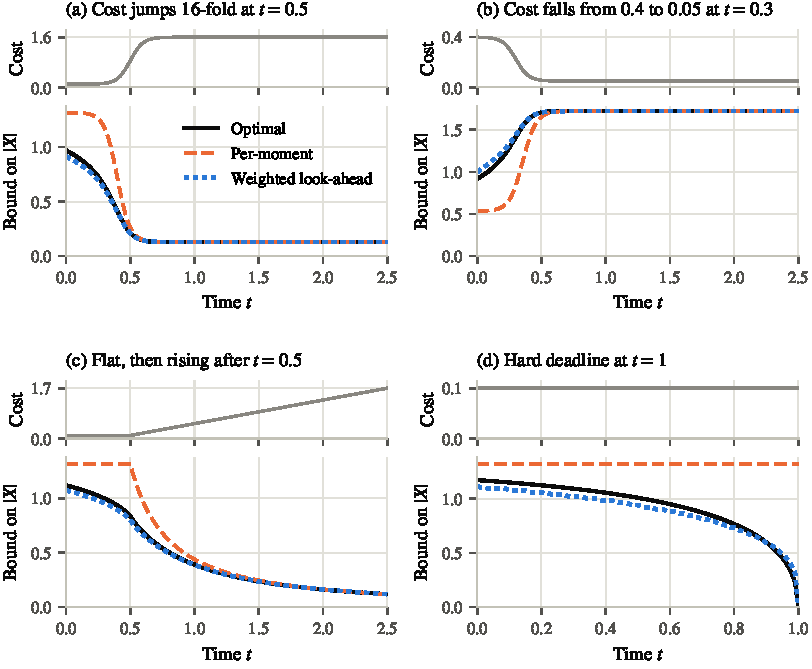
\includegraphics[width=\linewidth]{figures/showcase.pdf}
  \caption{Optimal bound (black), per-moment rule (orange, dashed), and weighted look-ahead rule
    (blue, dotted) for four cost schedules, in units where $\mu = \sigma = 1$; the strip above each panel is the cost
    $c(t)$. (a) The cost rises from 0.1 to 1.6 in a step centered at $t = 0.5$. (b) It falls from 0.4
    to 0.05 in a step centered at $t = 0.3$. Both steps are logistic in time, with scale 0.05. (c) It is 0.1, then $0.1 + 0.8\,(t - 0.5)$ after $t = 0.5$. (d) It is 0.1 until a
    deadline at $t = 1$, the right edge. The per-moment rule
    reacts to a change only when it arrives. The optimal bound starts moving earlier, and the
    weighted rule tracks it. Losses are in \cref{tab:showcase}.}
  \label{fig:showcase}
\end{figure}

\section{An exact equation for the bound}
\label{sec:exact}

\paragraph{Structure.}
The first lemma collects what follows from comparison arguments alone.

\begin{lemma}[Structure]
\label{lem:structure}
\begin{enumerate}
  \item[(a)] For each $t$, $y \mapsto V(t, y) - g(y)$ is nonincreasing, so the stopping set at time
    $t$ is an interval $[b(t), \infty)$.
  \item[(b)] If $c_1 \le c_2$ pointwise, then $V^{c_1} \ge V^{c_2}$ and $b^{c_1} \ge b^{c_2}$.
  \item[(c)] Hence $B(c_{\max}) \le b(t) \le B(c_{\min})$ for all $t$.
  \item[(d)] $|V(t, y) - V(t', y)| \le (c_{\max} - c_{\min})|t - t'|$ for all $t, t', y$.
\end{enumerate}
\end{lemma}

Part (d) holds for any bounded measurable cost: for a fixed stopping time $\tau$, the costs paid
from start times $t$ and $t'$ differ by at most $(c_{\max} - c_{\min})|t - t'|$, pathwise. Write
\begin{equation}
  \tau^*_{t,y} = \inf\{s \ge 0 : Y_s \ge b(t+s)\}, \qquad Y_0 = y,
\end{equation}
for the first entry into the stopping set from $(t, y)$; it is an optimal stopping time, by the
standing facts at the start of \cref{app:proofs}.

\paragraph{The envelope identity.}
In the continuation region, the value is smooth and satisfies the backward equation
$V_t + \Lop V = c$. The time derivative has a simple form.

\begin{lemma}[Envelope identity]
\label{lem:envelope}
At every point $(t, y)$ with $0 \le y < b(t)$, $V$ is smooth in $y$ and continuously
differentiable in $t$, $V_y(t, 0) = 0$, and
\begin{equation}
  V_t(t, y) = c(t) - \E_y\bigl[c(t + \tau^*_{t,y})\bigr], \qquad
  \Lop V(t, y) = \E_y\bigl[c(t + \tau^*_{t,y})\bigr].
  \label{eq:envelope}
\end{equation}
\end{lemma}

The first identity is an envelope theorem: if the optimal stopping time from $(t, y)$ is held
fixed while the start time moves, the reward it earns is a lower bound for $V$ that touches it at
$t$, so the two have the same derivative there, and that derivative only involves the cost paid at
the start and at the end. With $V_t + \Lop V = c$, it gives the second identity. In words, the
value's curvature term $\Lop V$, which equals $c$ for a constant cost, is the expected cost
at the moment of decision.

\paragraph{Regularity.}
Write $W = V - g \ge 0$ for the value of being allowed to wait. On $[0, b(t))$,
$\Lop W = \Lop V \ge c_{\min}$ by \eqref{eq:envelope}, and $W$ is nonincreasing by
\cref{lem:structure}(a). Integrating $(\cosh^2 y\,W_y)' = 2\cosh^2 y\,\Lop W$ shows that $W$ grows at
least quadratically away from the bound. Combined with the Lipschitz bound in time, this pins
down the bound's regularity.

\begin{proposition}[Regularity]
\label{prop:regularity}
\begin{enumerate}
  \item[(a)] \emph{Nondegeneracy.} $W(t, y) \ge c_{\min}\,(b(t) - y)^2$ for $0 \le y \le b(t)$.
  \item[(b)] \emph{Hölder continuity.}
    $|b(t) - b(t')| \le \sqrt{(c_{\max} - c_{\min})/c_{\min}}\;|t - t'|^{1/2}$ for all $t, t' \ge 0$.
  \item[(c)] \emph{Smooth fit.} For every $t \ge 0$, $V_y(t, y) \to g'(b(t))$ as $y \uparrow b(t)$.
\end{enumerate}
\end{proposition}

Part (b) follows from (a) and \cref{lem:structure}(d) in one line: if $b(t') > b(t)$, the point
$y = b(t)$ has $W(t, y) = 0$ and $W(t', y) \ge c_{\min}(b(t') - b(t))^2$, while the two differ by
at most $(c_{\max} - c_{\min})|t - t'|$. Part (c) uses (b): since the bound can rise by at most a
constant times $\sqrt{s}$ in time $s$, the law of the iterated logarithm makes the evidence cross
it immediately from any boundary point, and a coupling argument then gives smooth fit. This is
the one-dimensional case of the mechanism of \citet{deangelis2020}, who derive smooth fit from
the probabilistic regularity of boundary points alone.

\paragraph{The exact equation.}
Multiply the second identity in \eqref{eq:envelope} by $2\cosh^2 y$, integrate from the reflecting
center to the bound, and use smooth fit with $\cosh^2 b\; g'(b) = \tfrac12$.

\begin{proposition}[Exact equation for the bound]
\label{prop:exact}
For every $t \ge 0$,
\begin{equation}
  \int_0^{b(t)} \cosh^2 y\;\E_y\bigl[c(t + \tau^*_{t,y})\bigr]\dd y = \frac14.
  \label{eq:exact}
\end{equation}
\end{proposition}

For a constant cost, the left side is $c\,(\tfrac12 b + \tfrac14\sinh 2b)$, and \eqref{eq:exact}
is \eqref{eq:constant-bound}. In general, the equation says that the bound sits where the
$\cosh^2$-weighted average, over evidence levels below it, of the expected cost at the moment of
decision equals what a constant cost would require. It involves no derivative of the bound, which
makes it convenient to linearize.

\begin{remark}[Scale and speed]
\label{rem:speed}
The weight $\cosh^2 y$ is half the speed density of $Y$. For a diffusion with generator
$\tfrac12 f'' + \mu f'$, scale density $s' = \exp(-\int 2\mu)$, and speed density $m = 2/s'$, one has
$(f'/s')' = m\,\Lop f$; here $s' = \sech^2 y$ and $m = 2\cosh^2 y$. Because the reward is harmonic,
$g'/s'$ is constant, equal to $\tfrac12$, and the same steps give
$\int_0^{b(t)} m(y)\,\E_y[c(t + \tau^*_{t,y})]\dd y = g'/s'$. So \eqref{eq:exact} is an instance
of a general identity for one-dimensional problems with a harmonic reward, and
\cref{lem:kernel}(b) says the kernel is the decision time started from the normalized speed
measure on $[0, b_0]$. \Cref{sec:extensions} uses this for unknown reliability.
\end{remark}

\section{First-order theory}
\label{sec:first-order}

\subsection{The kernel}

Let $\tau_0$ be the first time $Y$ reaches $b_0 = B(c_0)$, which is the first exit time of $X$
from $(-b_0, b_0)$. Define the survival flux at the bound and its normalization,
\begin{equation}
  n(s) = -\partial_x \P_x(\tau_0 > s)\big|_{x = b_0}, \qquad
  w(s) = \frac{n(s)}{\int_0^\infty n(u)\dd u}.
  \label{eq:kernel}
\end{equation}
For a bounded function $\gamma$, write
\begin{equation}
  (w \star \gamma)(t) = \int_0^\infty w(s)\,\gamma(t+s)\dd s.
\end{equation}

\begin{lemma}[Two descriptions of the kernel]
\label{lem:kernel}
\begin{enumerate}
  \item[(a)] $n$ is positive and has the series
    \begin{equation}
      n(s) = \frac{2}{b_0}\sum_{j \ge 0} \frac{\kappa_j^2}{1 + \kappa_j^2}\,
      e^{-(1 + \kappa_j^2)s/2}, \qquad \kappa_j = \frac{(j + \frac12)\pi}{b_0},
      \label{eq:series}
    \end{equation}
    with $\int_0^\infty n = \tanh b_0 + b_0\sech^2 b_0 = 1/(2c_0\cosh^2 b_0)$.
  \item[(b)] $w$ is the density of $\tau_0$ when $Y_0$ is drawn from the density
    $\pi_0(y) = 4c_0\cosh^2 y$ on $[0, b_0]$:
    \begin{equation}
      w(s)\dd s = \int_0^{b_0} \pi_0(y)\,\P_y(\tau_0 \in \dd s)\dd y.
      \label{eq:mixture}
    \end{equation}
  \item[(c)] Its Laplace transform is
    $\tilde w(\lambda) = 2c_0\cosh^2 b_0\,[\,r\tanh(rb_0) - \tanh b_0\,]/\lambda$, with
    $r = \sqrt{2\lambda + 1}$, as in \eqref{eq:transfer-intro}.
\end{enumerate}
\end{lemma}

That $\pi_0$ integrates to one is \eqref{eq:constant-bound} again. Description (b) explains the
kernel's shape. Most of the weight of $\pi_0$ lies within a distance of order one below the bound,
since $\cosh^2 y$ grows like $e^{2y}$, and decisions that start there end soon. As $c_0 \to 0$,
$b_0 - Y_0$ becomes exponential with rate 2, the drift near the bound is nearly 1, and the
expected time to cover that distance tends to $\tfrac12$, which is the limit of the mean
look-ahead below.

\subsection{The theorem}

\begin{theorem}
\label{thm:main}
Let $\gamma$ be continuous with $|\gamma| \le M$, let $c_\varepsilon = c_0 + \varepsilon\gamma$,
and let $b_\varepsilon$ be the optimal bound for $c_\varepsilon$. Then, as $\varepsilon \to 0$,
\begin{equation}
  \frac{b_\varepsilon(t) - b_0}{\varepsilon} \longrightarrow \beta(t) := B'(c_0)\,(w \star \gamma)(t)
\end{equation}
uniformly for $t$ in compact sets, and uniformly on $[0, \infty)$ if $\gamma$ is uniformly
continuous. If $\gamma$ is Hölder continuous with exponent $\alpha \in (0, 1]$, then
$b_\varepsilon(t) = b_0 + \varepsilon\beta(t) + O(|\varepsilon|^{1+\alpha})$ uniformly on
$[0, \infty)$; in particular, the remainder is $O(\varepsilon^2)$ when $\gamma$ is Lipschitz.
\end{theorem}

\begin{proof}[Proof sketch]
Apply \eqref{eq:exact} to $c_\varepsilon$ and subtract its constant-cost version. With
$F(b) = \int_0^b \cosh^2 y\dd y$,
\begin{equation}
  c_0\bigl[F(b_\varepsilon(t)) - F(b_0)\bigr]
  = -\varepsilon\int_0^{b_\varepsilon(t)} \cosh^2 y\;\E_y\bigl[\gamma(t + \tau^\varepsilon_{t,y})\bigr]\dd y.
\end{equation}
By \cref{lem:structure}(c), $|b_\varepsilon - b_0| \le a|\varepsilon|$ for a constant $a$, so
$\tau^\varepsilon_{t,y}$ lies between the hitting times of the fixed levels $b_0 \pm a|\varepsilon|$,
and both converge to $\tau_0$ almost surely. Dividing by $\varepsilon$, dominated convergence gives
\begin{equation}
  c_0\cosh^2 b_0\,\frac{b_\varepsilon(t) - b_0}{\varepsilon} \to
  -\int_0^{b_0}\cosh^2 y\;\E_y\bigl[\gamma(t + \tau_0)\bigr]\dd y
  = -\frac{1}{4c_0}(w \star \gamma)(t),
\end{equation}
by \eqref{eq:mixture}, and $-1/(4c_0^2\cosh^2 b_0) = B'(c_0)$. \Cref{app:proofs} gives the details
and the uniformity.
\end{proof}

\subsection{Closed forms}

\begin{corollary}[Transfer function]
\label{cor:transfer}
For a sinusoidal cost $\gamma(t) = \operatorname{Re}(\Gamma e^{i\omega t})$ with $\omega > 0$,
\begin{equation}
  \beta(t) = \operatorname{Re}\bigl(B'(c_0)\,\tilde w(-i\omega)\,\Gamma\,e^{i\omega t}\bigr).
\end{equation}
So the bound's swing is $|\tilde w(-i\omega)| < 1$ times the swing of the per-moment response
$B'(c_0)\gamma$, and the bound leads that response by the phase $\arg\tilde w(-i\omega) \in
(0^\circ, 90^\circ)$.
\end{corollary}

The signs come from the series \eqref{eq:series}: $\tilde w(-i\omega)$ is a positive combination
of terms $1/(\alpha_j - i\omega)$ with $\alpha_j > 0$, each with positive real and imaginary
parts.

\begin{corollary}[Limits]
\label{cor:limits}
\begin{enumerate}
  \item[(a)] \emph{Slow changes.} $\tilde w(0) = 1$, so very slow changes recover the per-moment
    rule.
  \item[(b)] \emph{Mean look-ahead.} The mean of $w$ is
    \begin{equation}
      m(c_0) = -\tilde w'(0) = c_0\Bigl[\tfrac12\sinh(2b_0) - b_0 + 2b_0^2\tanh b_0\Bigr]
      = \frac12 + \frac{2b_0(b_0\tanh b_0 - 1)}{\sinh 2b_0 + 2b_0}.
      \label{eq:mean-look-ahead}
    \end{equation}
    It is the mean of $\tau_0$ under the start $\pi_0$, with $\E_y\tau_0 = b_0\tanh b_0 - y\tanh y$.
    It tends to $\tfrac12$ as $c_0 \to 0$ and to 0 as $c_0 \to \infty$, and numerically its
    maximum over $c_0$ is about $\MaxLookAhead$, at $c_0 \approx \MaxLookAheadCost$. For a cost
    that changes slowly and nearly linearly over the decision's time scale, the optimal bound at
    $t$ is, to first order, close to the per-moment bound for the cost at $t + m(c_0)$.
  \item[(c)] \emph{Fast changes.} As $\omega \to \infty$,
    $|\tilde w(-i\omega)| \sim 2c_0\cosh^2(b_0)\sqrt{2/\omega}$ and
    $\arg\tilde w(-i\omega) \to 45^\circ$.
\end{enumerate}
\end{corollary}

In original units, the look-ahead stays below about $\MaxLookAhead\,\sigma^2/\mu^2$. When time is
nearly free, the decision maker deliberates for a long time, with mean decision time
$b_0\tanh b_0 \to \infty$, yet the bound looks only about half a time unit ahead, because the
weights $\pi_0$ concentrate near the bound. At $c_0 = 0.1$, the look-ahead is $\LookAheadTenth$
against a mean decision time of $\DecisionTimeTenth$. Part (c) says the kernel behaves like
$s^{-1/2}$ near $s = 0$, a half-integration, so fast cost fluctuations are smoothed but not
ignored. \Cref{fig:kernels,fig:transfer} show the kernels, the look-ahead, and the transfer
function.

\begin{figure}[t]
  \centering
  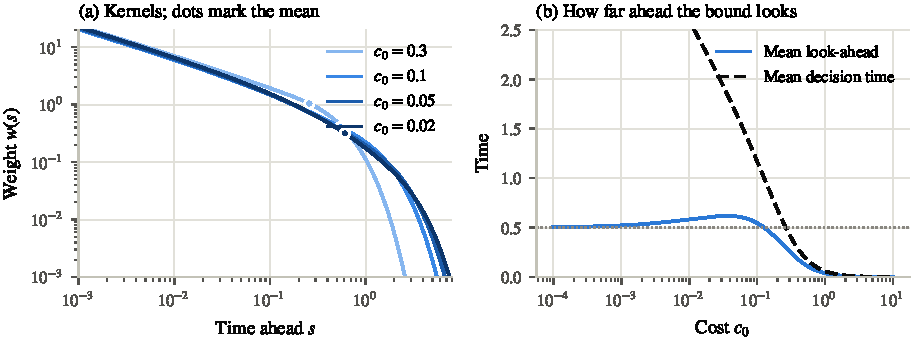
\includegraphics[width=\linewidth]{figures/kernels.pdf}
  \caption{(a) The kernel $w(s)$ for four costs, on log axes; dots mark the mean look-ahead
    $m(c_0)$. Near $s = 0$, the kernel behaves like $s^{-1/2}$. (b) The mean look-ahead
    \eqref{eq:mean-look-ahead} stays below about $\MaxLookAhead$ for every cost and tends to
    $\tfrac12$ (dotted) as time becomes free, while the mean decision time $b_0\tanh b_0$ grows
    without bound.}
  \label{fig:kernels}
\end{figure}

\begin{figure}[t]
  \centering
  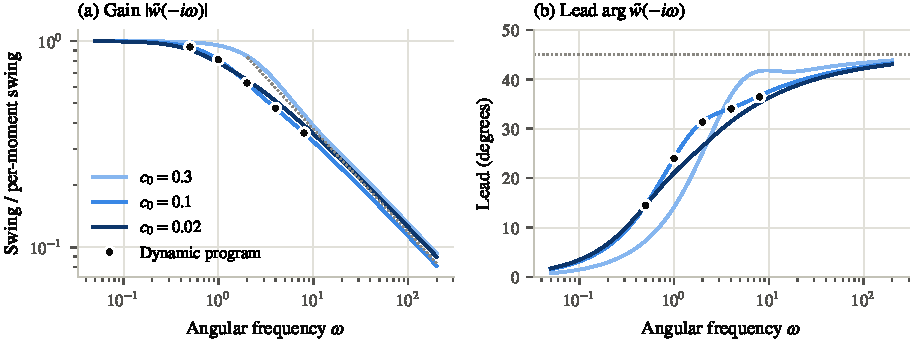
\includegraphics[width=\linewidth]{figures/transfer.pdf}
  \caption{The transfer function $\tilde w(-i\omega)$ for three costs. (a) The bound's swing in
    response to a sinusoidal cost, relative to the per-moment swing; the dotted line is the
    high-frequency asymptote for $c_0 = 0.1$. (b) The phase lead over the per-moment response,
    which tends to $45^\circ$. Dots: the dynamic program for $c_0 = 0.1$ and $\varepsilon = 0.01$
    (\cref{tab:sinusoid}).}
  \label{fig:transfer}
\end{figure}

\subsection{How much reward a nearby rule loses}
\label{sec:loss}

A bound that misses the optimum loses reward only at second order, because the expected reward is
flat at the optimum. Near a constant cost, this holds uniformly over rules.

\begin{proposition}[Second-order loss]
\label{prop:loss}
Fix a starting point $y_0 \in [0, b_0)$ and $a > 0$. There is a constant $C$ such that, for all
small $\varepsilon$, every policy that stops when $Y$ first reaches a continuous bound $\hat b$ with
$\|\hat b - b_0\|_\infty \le a|\varepsilon|$ earns at most $C\varepsilon^2$ less than the optimal
policy for the cost $c_0 + \varepsilon\gamma$.
\end{proposition}

The per-moment rule and the weighted look-ahead both qualify, so both lose $O(\varepsilon^2)$. The
proof (\cref{app:proofs}) combines quadratic contact at the bound, $W \le C(b - y)^2$, with the
fact that the time spent in a band of width $D$ next to an absorbing level is $O(D^2)$. A sharper
statement would say how much each rule loses.

\begin{conjecture}[Leading-order loss]
\label{conj:loss}
Let $f$ be bounded and Lipschitz. A policy whose bound misses the optimum by
$\eta = \varepsilon f$ loses
\begin{equation}
  \E\bigl[c(\hat\tau)\,\eta(\hat\tau)^2\bigr]
  \label{eq:loss}
\end{equation}
up to $o(\varepsilon^2)$, where $\hat\tau$ is its decision time.
\end{conjecture}

The constant agrees with two exact facts: on the continuation side of the bound, $(V - g)_{yy} = 2c(t)$, and at a
constant cost the reward of a flat bound $b$, $g(b) - c\,b\tanh b$, has curvature exactly $-2c$ at
$b = B(c)$. \Cref{sec:loss-check} checks the formula numerically. \Cref{prop:loss} already bounds both rules' losses by $O(\varepsilon^2)$. The conjecture
concerns a fixed miss $\varepsilon f$, while the rules' misses change shape with $\varepsilon$, so
it does not by itself say how much less the weighted rule loses. Heuristically, a loss quadratic
in the miss would make the per-moment rule lose order $\varepsilon^2$ and the weighted rule, which
misses by $O(\varepsilon^2)$ for a smooth change (\cref{prop:rule}), order $\varepsilon^4$;
\cref{sec:loss-check} measures how fast it actually falls.

\section{The weighted look-ahead rule}
\label{sec:rule}

\Cref{thm:main} and \cref{prop:rule} below cover small changes in a continuous cost, bounded
between two positive constants, on an infinite horizon. Large steps, deadlines, and the forced
choice at $t = 10$ in our experiments lie outside them. There, the rules of this section are
heuristics motivated by the theorem, and we judge them by measurement (\cref{sec:experiments}).
\Cref{fig:showcase}(d) shows what that means on a deadline: the weighted rule's bound sits below
the optimal one for most of the trial, then above it from about $t = 0.9$ to the deadline, by
up to about 0.1.

\Cref{thm:main} suggests two rules that need no dynamic program. The first replaces the cost by
its weighted average,
\begin{equation}
  b_{\mathrm{avg}}(t) = B\bigl((w_{c(t)} \star c)(t)\bigr),
\end{equation}
where $w_c$ is the kernel for the constant cost $c$. It is exact to first order, but it fails
when the cost becomes infinite, as it does past a deadline. The second averages the per-moment
bounds themselves.

\begin{definition}[Weighted look-ahead]
For a level $b > 0$, let $w_b$ be the kernel \eqref{eq:kernel} computed for the interval
$(-b, b)$, and let $w_0$ be a unit mass at $s = 0$. The weighted look-ahead bound $b_{\mathrm{w}}(t)$
solves
\begin{equation}
  b_{\mathrm{w}}(t) = \int_0^\infty w_{b_{\mathrm{w}}(t)}(s)\, B\bigl(c(t+s)\bigr)\dd s,
  \label{eq:weighted}
\end{equation}
with $B(\infty) = 0$, so that $b_{\mathrm{w}} = 0$ at and after a deadline.
\end{definition}

\begin{proposition}[Near a constant cost, the rule is well defined and first-order exact]
\label{prop:rule}
For $c = c_0 + \varepsilon\gamma$ with $\gamma$ continuous, $|\gamma| \le M$, and $|\varepsilon|$
small, \eqref{eq:weighted}
has a unique solution in $[B(c_0 + |\varepsilon|M), B(c_0 - |\varepsilon|M)]$ at each $t$, and
\begin{equation}
  b_{\mathrm{w}}(t) = b_0 + \varepsilon\beta(t) + O(\varepsilon^2)
\end{equation}
uniformly in $t$. Hence $(b_{\mathrm{w}} - b_\varepsilon)/\varepsilon \to 0$ locally uniformly,
while $(b_{\mathrm{pm}} - b_\varepsilon)/\varepsilon \to B'(c_0)(\gamma - w \star \gamma)$, which is
not identically zero unless $\gamma$ is constant. If $\gamma$ is Lipschitz,
$b_{\mathrm{w}} - b_\varepsilon = O(\varepsilon^2)$ uniformly.
\end{proposition}

The key step is that every $w_b$ integrates to one, so changing the kernel moves the average of a
nearly constant function only at second order; this makes the right side of
\eqref{eq:weighted} a contraction in $b_{\mathrm{w}}(t)$. For large changes, the equation can have
more than one solution: a cost that is high for a short time and then low can make both a small
and a large level self-consistent. In the experiments, the rule is the output of the iteration below,
started from the per-moment bound; for large and fast changes, 30 updates need not reach a solution
of \eqref{eq:weighted}, so this is an implemented approximation and not a selected root. 
The two rules
agree to first order, but
they differ for large changes. A cost spike can pull the optimal bound only down to zero, and
averaging bounds respects that; averaging costs does not. Past a deadline $T$, the cost is
infinite, making $B(c(t+s)) = 0$ for $s > T - t$, and the bound collapses smoothly toward the
deadline (\cref{fig:showcase}d). No special case is needed.

\paragraph{Computation.}
We solve \eqref{eq:weighted} by damped fixed-point iteration: start from the per-moment bound and
replace $b_{\mathrm{w}}$ by the average of itself and the right side, 30 times
(\cref{alg:weighted}). Kernels come from their eigenfunction series, on a grid of bound levels with
spacing $10^{-3}$; each is built the first time its level is needed and then cached, and levels
below 0.01 use the kernel for 0.01. Each update then costs one weighted sum over 240 future times
at each time point. On our code, the rule is not faster than the dynamic program. In our timings of a dozen schedules
on one computer, the dynamic program took 0.03--0.6~s per schedule and the rule 0.1--1.7~s with its
kernels cached, and a first call that builds the kernels took up to about 16~s. What the rule
offers is an explanation, not speed: it says how far ahead the bound looks and with what weights.

\begin{algorithm}[t]
  \caption{The weighted look-ahead rule as computed in the experiments.}
  \label{alg:weighted}
  \begin{algorithmic}[1]
    \Require a cost $c(t)$ that can be evaluated at any $t \ge 0$ (not only on the grid
      $t_k = k\,\Delta t$); constant-cost bound $B(c)$, from a 2001-point table in $\log c$ on
      $[10^{-5}, 10^{4}]$, finite costs clipped to that range, and $B(\infty) = 0$
    \State $b(t_k) \gets B(c(t_k))$ for every $k$ \Comment{per-moment start}
    \For{$i = 1, \dots, 30$}
      \For{each $k$}
        \State $\ell \gets \max(b(t_k), 0.01)$ rounded to $10^{-3}$
        \State $(s_j, w_j)_{j \le 240} \gets$ kernel bins for the bound $\ell$ \Comment{built once per $\ell$, then cached}
        \State $a(t_k) \gets \sum_j w_j\, B\bigl(c(t_k + s_j)\bigr)$
      \EndFor
      \State $b \gets \tfrac12 (b + a)$ \Comment{damped update}
    \EndFor
    \State \Return $\max\bigl(b(t_k) - 0.5826\sqrt{\Delta t},\, 0\bigr)$ for every $k$ \Comment{discrete monitoring}
  \end{algorithmic}
  \smallskip
  \footnotesize The kernel for $\ell$ is the survival flux of \eqref{eq:kernel} on $(-\ell, \ell)$,
  from 4000 terms of its eigenfunction series. It is integrated exactly over 240 bins with edges
  $0$ and 240 geometrically spaced points from $10^{-5}$ to $14/\lambda_1$, where
  $\lambda_1 = \tfrac12\bigl((\pi/2\ell)^2 + 1\bigr)$; so the first bin is $[0, 10^{-5}]$, which holds
  a quarter of the mass at $\ell = 0.01$. The bin masses are normalized to sum to one as $w_j$, and
  $s_j$ is each bin's midpoint.
\end{algorithm}

\section{Experiments}
\label{sec:experiments}

\subsection{Methods}
\label{sec:methods}

\paragraph{The reference.}
For each cost schedule, we compute the optimal policy by backward induction on an evidence grid
with spacing $h = 0.005$ and time step $\Delta t = 0.002$, truncated at $|x| = 8$. The expected
value of waiting at each grid point is a mixture of two Gaussian convolutions, one for each drift,
weighted by the posterior $g(x)$, and computed with the fast Fourier transform. The choice is
forced at the last grid time, and schedules without a deadline end with a forced choice at
$t = 10$. Compared to the decision times involved, this horizon is long, but it does change the
problem slightly: at a constant cost of 0.02, about one decision in a thousand is still undecided
at $t = 10$ under the constant-cost bound, which as a result loses \HorizonFloor{} points per 100
trials against the optimum for that horizon. The heuristic rules are not given this $t = 10$
cutoff; they treat the horizon as infinite.

\paragraph{Scoring.}
A policy is a bound $\hat b(t)$ on the evidence grid. We score it deterministically on the grid,
without Monte Carlo: we propagate the evidence density forward on the same grid under the drift $+1$, which suffices
by symmetry, absorb the mass that
crosses the bound, and add up the reward of each decision and the cost of the time spent. Losses
are reported in points per 100 trials,
$100 \times (\text{reward of the optimal policy} - \text{reward of the policy})$. Because the
reference is the best policy on the scorer's own grid, losses are nonnegative up to the
interpolation of bounds between grid points; the few negative entries are tiny. We have not
bounded the grid's own discretization error. On eight development schedules, refining the grid to
a quarter of the time step and half the spacing moves the losses by at most \GridPmMaxChange{}
(\cref{tab:grid}).

\paragraph{Discrete monitoring.}
The cheap rules give bounds for continuous monitoring, but the grid checks the bound every
$\Delta t$. To leading order as $\Delta t \to 0$, the optimal boundary of a sequential test checked
at intervals $\Delta t$ sits $0.5826\,\sigma\sqrt{\Delta t}$ inside the continuous one, where
$0.5826 = -\zeta(\tfrac12)/\sqrt{2\pi}$ \citep{chernoff1965}; the same constant governs the
overshoot of a discretely monitored barrier \citep{siegmund1979,broadie1997}, so before
scoring, we move each continuous bound inward by that amount. The dynamic program needs no
correction, since it is solved on the grid itself.

\subsection{The first-order theory against the dynamic program}
\label{sec:sinusoid}

We set $c_0 = 0.1$ and $\gamma(t) = \sin(\omega t)$ with $\varepsilon = 0.01$, for five
frequencies, solve each problem by dynamic programming over beliefs (800 belief bins), and fit a
sinusoid to the bound's deviation from $b_0$ over whole periods from $t = 2$: at least two periods
and at least 6 time units, with the horizon 6 time units after the end of the fit.
\Cref{tab:sinusoid} and \cref{fig:transfer} compare the swing and the lead with the closed form
\eqref{eq:transfer-intro} and with the weighted look-ahead rule $b_{\mathrm{w}}$. At every
frequency, the closed form agrees with the dynamic program to about \ClosedFormWorstGain\% on the
swing and \ClosedFormWorstLead$^\circ$ on the lead, and the weighted rule to about
\SinusoidWorstGain\% and \SinusoidWorstLead$^\circ$. The per-moment rule's swing is
\PerMomentTooLargeAtEight{} times too large at $\omega = 8$, and it lags by
\PerMomentLateAtEight$^\circ$.

\Cref{tab:sweep} tests \cref{thm:main} more widely, at three costs, two frequencies, and four sizes
of the perturbation, against the exact policy on a finer evidence grid. The fitted swing differs
from the predicted one by at most about \SweepSwingTenth\% at $\varepsilon/c_0 = 0.1$, \SweepSwingThird\% at 0.3, and
\SweepSwingSixTenths\% at 0.6, so the error shrinks about like $(\varepsilon/c_0)^2$; the phase, by
at most about \SweepPhaseTenth$^\circ$, \SweepPhaseThird$^\circ$, and \SweepPhaseSixTenths$^\circ$.


\begin{table}[t]
  \centering
  \caption{Response of the bound to a sinusoidal cost, $c_0 = 0.1$, $\varepsilon = 0.01$. Swing is
    relative to the per-moment swing, and lead is in degrees ahead of the per-moment response.}
  \label{tab:sinusoid}
  \begin{tabular}{rrrrrrr}
    \toprule
    & \multicolumn{2}{c}{Closed form} & \multicolumn{2}{c}{Dynamic program} & \multicolumn{2}{c}{Weighted look-ahead} \\
    \cmidrule(lr){2-3} \cmidrule(lr){4-5} \cmidrule(lr){6-7}
    $\omega$ & Swing & Lead & Swing & Lead & Swing & Lead \\
    \midrule
    \inputrows{generated/tab_sinusoid.tex}
    \bottomrule
  \end{tabular}
\end{table}

\begin{table}[t]
  \centering
  \caption{\Cref{thm:main} against the exact policy for $c(t) = c_0 + \varepsilon \sin(\omega t)$:
    fitted swing over predicted swing, the range over $\omega \in \{1, 4\}$, and the largest
    phase error. Exact policy on the evidence grid ($h = 0.0025$, horizon 14), fit on
    $2 < t < 2 + 2\pi$.}
  \label{tab:sweep}
  \begin{tabular}{rrrrr}
    \toprule
    $\varepsilon/c_0$ & $c_0 = 0.03$ & $c_0 = 0.1$ & $c_0 = 0.3$ & Phase error ($^\circ$) \\
    \midrule
    \inputrows{generated/tab_sweep.tex}
    \bottomrule
  \end{tabular}
\end{table}

\subsection{Random cost schedules}
\label{sec:random}

We drew 90 development schedules from seed 2026, the seed used while the rule was designed, 30 in
each of three families:
\begin{itemize}
  \item \emph{Smooth}: $\log c(t) = \log c_0 + \sum_{j=1}^3 a_j \sin(\omega_j t + \phi_j)$, with
    $c_0$ log-uniform on $[0.02, 0.5]$, $a_j$ uniform on $[-\tfrac23, \tfrac23]$, $\omega_j$
    uniform on $[0.3, 6]$, and $\phi_j$ uniform.
  \item \emph{Step}: a jump from $c_0$ to $c_0 r$ at time $t_0$, logistic in time with scale 0.05, with $c_0$
    log-uniform on $[0.02, 1]$, $r$ log-uniform on $[\tfrac1{16}, 16]$, and $t_0$ uniform on
    $[0.1, 2]$.
  \item \emph{Deadline}: a constant cost $c_0$, log-uniform on $[0.01, 0.5]$, and a forced choice
    at $T$, uniform on $[0.3, 3]$.
\end{itemize}
\Cref{tab:random} and \cref{fig:random} report the losses. The per-moment rule loses up to
\PerMomentMaxAll{} points per 100 trials; the weighted look-ahead loses at most \WeightedMaxAll.
Measured as total loss, the weighted rule recovers \RecoveredSmooth\% of the per-moment rule's
loss on smooth schedules, \RecoveredStep\% on steps, and \RecoveredDeadline\% on deadlines.
\Cref{tab:showcase} gives the losses for the four schedules of \cref{fig:showcase}.

\begin{table}[t]
  \centering
  \caption{Losses in points per 100 trials on the 90 development schedules. ``Recovered'' is the share of
    the per-moment rule's total loss that the weighted look-ahead avoids.}
  \label{tab:random}
  \begin{tabular}{lrrrrrr}
    \toprule
    & & \multicolumn{2}{c}{Per-moment} & \multicolumn{2}{c}{Weighted look-ahead} & \\
    \cmidrule(lr){3-4} \cmidrule(lr){5-6}
    Family & $n$ & Median & Max & Median & Max & Recovered \\
    \midrule
    \inputrows{generated/tab_random.tex}
    \bottomrule
  \end{tabular}
\end{table}

\begin{figure}[t]
  \centering
  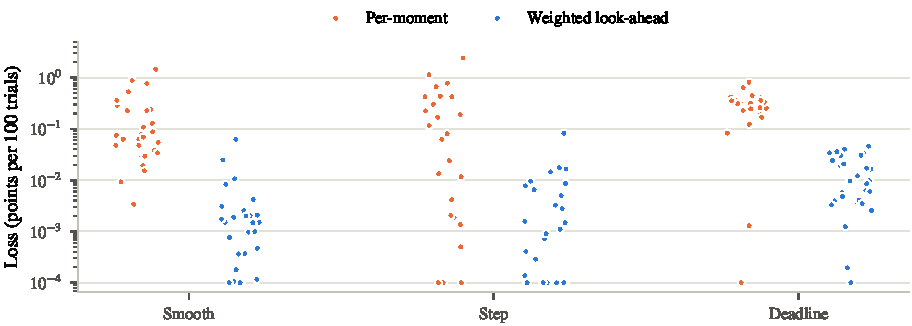
\includegraphics[width=\linewidth]{figures/random_losses.pdf}
  \caption{Loss of each rule on each of the 90 development schedules, on a log scale. Losses below
    $10^{-4}$, including the schedules where both rules are optimal to grid precision, are drawn
    at $10^{-4}$.}
  \label{fig:random}
\end{figure}

\begin{table}[t]
  \centering
  \caption{Losses in points per 100 trials for the schedules in \cref{fig:showcase}.}
  \label{tab:showcase}
  \begin{tabular}{lrr}
    \toprule
    Schedule & Per-moment & Weighted look-ahead \\
    \midrule
    \inputrows{generated/tab_showcase.tex}
    \bottomrule
  \end{tabular}
\end{table}

\subsection{Held-out schedules and other rules}
\label{sec:heldout}

The 90 schedules of \cref{sec:random} come from the seed used while the rule was designed, so they
are a development set. To test the rule on schedules it was not shaped by, we specified a held-out
set before running it, and ran it once: seed 20261111, \HeldCount{} schedules, 30 in each of seven
families. Three families are those of \cref{sec:random}, and four are new:
\begin{itemize}
  \item \emph{Pulse}: a Gaussian bump in $\log c$ that changes the cost by up to 8-fold either
    way.
  \item \emph{Ramp}: $\log c$ changing linearly over a random time, so that the cost changes by up
    to 16-fold either way, then flat.
  \item \emph{Multi-step}: two to four steps, each changing the cost by up to 4-fold either way.
  \item \emph{Piecewise}: a cost constant on random intervals, about 0.45 time units long on
    average, at levels drawn independently and log-uniformly from $[0.02, 1]$.
\end{itemize}
Multi-step and piecewise schedules have their joins smoothed in $\log c$ by the same logistic. We also scored five more rules (\cref{tab:baselines}): the
weighted look-ahead after a single pass, with the kernel for the per-moment bound and no
iteration; the averaged-cost rule $b_{\mathrm{avg}}$; the per-moment rule shifted ahead by the mean
look-ahead, $B\bigl(c(t + m(c(t)))\bigr)$, and by half a time unit; and a constant bound tuned for
each schedule with the scorer itself, which is an oracle rather than a usable rule.

\Cref{tab:heldout} and \cref{fig:heldout} report the losses. The per-moment rule loses a median of
\HeldPerMomentMedian{} points per 100 trials (\HeldShareMedian\% of the reward) and at most
\HeldPerMomentMax; the weighted look-ahead loses at most \HeldWeightedMax. On the
\HeldRecoveredCount{} schedules where the per-moment rule loses at least 0.01, the weighted rule
recovers a median of \HeldRecoveredMedian\% of that loss, with a 10th percentile of
\HeldRecoveredPTen\% and a minimum of \HeldRecoveredMin\%; piecewise schedules are the hardest.
Away from deadlines, on the \HeldNoDeadlineCount{} schedules without one (a different set from
the \HeldRecoveredCount{} above, of the same size by coincidence), shifting the per-moment rule
by the mean look-ahead is worse than not shifting it on \HeldShiftMeanWorse{} schedules, so the kernel's shape
matters, not only its mean. Averaging costs instead of bounds beats the per-moment rule on
\HeldAveragedCostBeats{} of those \HeldNoDeadlineCount{} but fails on deadlines, as
\cref{sec:rule} predicts, with losses up to \HeldAveragedCostMax. A single pass of the weighted
rule loses up to \HeldOnePassMax, so the iteration matters in the worst cases. Even the tuned
constant bound beats the per-moment rule on only \HeldBestConstantBeats{} of the
\HeldNoDeadlineCount{} schedules without a deadline. \Cref{tab:behavior} reports how far each
rule's bound strays from the optimal one, and what that does to accuracy and decision time.

\begin{table}[t]
  \centering
  \small
  \caption{Held-out schedules: losses in points per 100 trials. ``Per schedule'' is the share of the
    per-moment rule's loss that the weighted rule avoids, over schedules where the per-moment rule
    loses at least 0.01 (median and 10th percentile); ``Totals'' is one minus the ratio of the
    family's total losses.}
  \label{tab:heldout}
  \begin{tabular}{lrrrrrrrr}
    \toprule
    & & \multicolumn{2}{c}{Per-moment} & \multicolumn{2}{c}{Weighted look-ahead} & \multicolumn{3}{c}{Recovered} \\
    \cmidrule(lr){3-4} \cmidrule(lr){5-6} \cmidrule(lr){7-9}
    Family & $n$ & Median & Max & Median & Max & Median & 10th pct. & Totals \\
    \midrule
    \inputrows{generated/tab_heldout.tex}
    \bottomrule
  \end{tabular}
\end{table}

\begin{table}[t]
  \centering
  \small
  \caption{Held-out schedules: losses of seven rules in points per 100 trials, on the
    \HeldNoDeadlineCount{} schedules without a deadline and on the 30 with one. ``Wins / losses''
    counts schedules on which a rule loses less or more than the per-moment rule. The tuned
    constant is a single evidence bound per schedule, chosen with the scorer itself by bounded
    scalar search on $[0.02, 4]$ with tolerance 0.005 (an oracle, not a usable rule).}
  \label{tab:baselines}
  \begin{tabular}{lrrrcrr}
    \toprule
    & \multicolumn{4}{c}{No deadline} & \multicolumn{2}{c}{Deadline} \\
    \cmidrule(lr){2-5} \cmidrule(lr){6-7}
    Rule & Median & 90th pct. & Max & Wins / losses & Median & Max \\
    \midrule
    \inputrows{generated/tab_baselines.tex}
    \bottomrule
  \end{tabular}
\end{table}

\begin{table}[t]
  \centering
  \small
  \caption{Held-out schedules, medians per family: the largest gap between each rule's bound and
    the optimal one before $t = 4$ (or the deadline), in evidence units; and the change in accuracy
    (percentage points) and in mean decision time (units of $\sigma^2/\mu^2$) relative to the
    optimal policy.}
  \label{tab:behavior}
  \begin{tabular}{lrrrrrr}
    \toprule
    & \multicolumn{2}{c}{Bound error} & \multicolumn{2}{c}{Accuracy change} & \multicolumn{2}{c}{Decision time change} \\
    \cmidrule(lr){2-3} \cmidrule(lr){4-5} \cmidrule(lr){6-7}
    Family & Per-moment & Weighted & Per-moment & Weighted & Per-moment & Weighted \\
    \midrule
    \inputrows{generated/tab_behavior.tex}
    \bottomrule
  \end{tabular}
\end{table}

\begin{figure}[t]
  \centering
  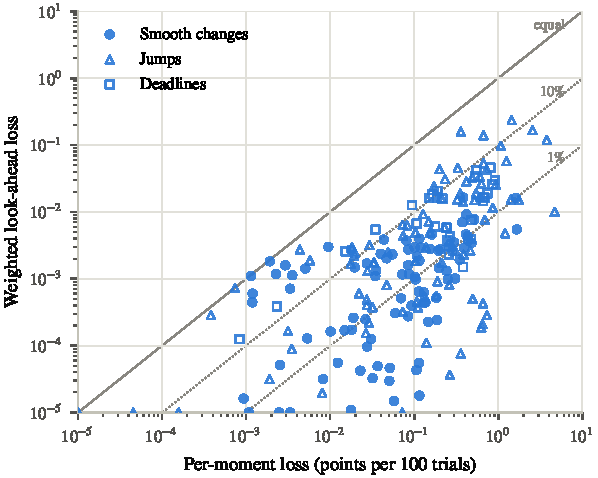
\includegraphics[width=0.62\linewidth]{figures/heldout_paired.pdf}
  \caption{Each held-out schedule's loss under the per-moment rule (horizontal) and the weighted
    look-ahead (vertical), on log scales; losses below $10^{-5}$ are drawn at $10^{-5}$. The lines
    mark equal loss and losses of 10\% and 1\% of the per-moment rule's.}
  \label{fig:heldout}
\end{figure}

\subsection{The loss formula}
\label{sec:loss-check}

To test \cref{conj:loss}, we computed the distribution of decision times for each rule exactly,
then predicted its loss as $\sum_j f_j\, c(t_j)\,\eta(t_j)^2$, where $f_j$ is the probability of
deciding at grid time $t_j$ and $\eta$ the rule's distance from the optimal bound. The sum leaves
out the last grid time, $t = 10$, where the scorer forces every undecided trial to choose whatever
either bound says, so a gap between the bounds there costs nothing. We used six smooth schedules at
each of three sizes and six steps at each of three ratios (seed 7), with base costs log-uniform on
$[0.03, 0.3]$. For a smooth schedule of size $a$, the three amplitudes of $\log c$ are uniform on
$[-\tfrac23 a, \tfrac23 a]$, with frequencies and phases drawn as in \cref{sec:random}; the steps
alternate up and down, at times uniform on $[0.2, 1.5]$. \Cref{tab:loss} shows that the formula
overestimates the per-moment rule's loss by \LossPmLow--\LossPmHigh\% for smooth schedules and for
steps up to threefold, and by \LossPmSixteen\% for 16-fold steps, where the bound error is no
longer small. For the weighted rule, whose total loss is about \LossTotalRatio{} times smaller, the
formula overestimates by a factor of \LossWbLow{} to \LossWbHigh. At the smallest size of each
family, most of that prediction comes from $t > 8$, where the optimal bound collapses toward the
forced choice at $t = 10$ and the rules, which ignore it, do not. There, the gap is not small, so
the formula need not hold; this part of the prediction comes from comparing rules that ignore the
horizon with the finite-horizon optimum (\cref{sec:methods}). So \cref{tab:loss} tests the formula
for the per-moment rule, but says little about the weighted rule.

Each row of \cref{tab:loss} also draws new schedules, so it cannot show how a loss scales with the
size of the change. \Cref{tab:scaling} does, for one smooth shape scaled in $\log c$ around
$c_0 = \ScalingCost$, where decisions are short and the forced choice at $t = 10$ hardly matters:
$c(t) = \ScalingCost\,e^{a f(t)}$ with $f(t) = 0.6\sin(1.3t + 0.4) + 0.5\sin(3.1t + 2) +
0.4\sin(5.2t + 4)$. We score each amplitude on the paper's grid and again on one twice as fine in time and
space. Up to $a = 0.4$, each doubling multiplies the per-moment rule's loss by
\ScalingPmGrowthLow{} to \ScalingPmGrowthHigh, close to the 4 of a second-order loss; its effective
order there is \ScalingPmOrder. The weighted rule's loss is far smaller, and only from $a = 0.2$ up
is it large enough for the two grids to agree on it, to within \ScalingGridChangeTwo\% at
$a = 0.2$ and better above; at the smallest amplitude, its sign even differs between them. From
$a = 0.2$ to 0.8, its effective order is \ScalingWbOrderLow{} on one grid and \ScalingWbOrderHigh{}
on the other. That is consistent with the heuristic fourth order of \cref{sec:loss}, but it is
a measurement over a short range, not an asymptotic result.


\begin{table}[t]
  \centering
  \caption{Total loss over six schedules per row (points per 100 trials), and the loss formula's
    prediction as a ratio to it.}
  \label{tab:loss}
  \begin{tabular}{llrrrr}
    \toprule
    & & \multicolumn{2}{c}{Per-moment} & \multicolumn{2}{c}{Weighted look-ahead} \\
    \cmidrule(lr){3-4} \cmidrule(lr){5-6}
    Family & Size & Loss & Predicted / actual & Loss & Predicted / actual \\
    \midrule
    \inputrows{generated/tab_loss.tex}
    \bottomrule
  \end{tabular}
\end{table}

\begin{table}[t]
  \centering
    \caption{Loss scaling for one smooth cost shape, $c(t) = \ScalingCost\,e^{a f(t)}$, in points per
    100 trials. ``Growth'' is the per-moment rule's loss over its loss at amplitude $a/2$; a
    second-order loss grows 4-fold per doubling. The weighted rule's loss is shown on the paper's
    grid and on one twice as fine in time and space; where the two differ widely, it is below what
    the grid resolves.}
  \label{tab:scaling}
  \begin{tabular}{lrrrr}
    \toprule
        & \multicolumn{2}{c}{Per-moment} & \multicolumn{2}{c}{Weighted look-ahead} \\
    \cmidrule(lr){2-3} \cmidrule(lr){4-5}
    $a$ & Loss & Growth & Loss & Finer grid \\
    \midrule
    \inputrows{generated/tab_scaling.tex}
    \bottomrule
  \end{tabular}
\end{table}

\section{Extensions}
\label{sec:extensions}

\subsection{Unknown evidence reliability}

Suppose the drift is not $\pm 1$ but $\mu \sim N(0, 1/a)$, drawn once per trial, with unit noise.
The decision maker's evidence is then the diffusion $\dd X = X/(t + a)\dd t + \dd\bar W$, and the
posterior probability that $\mu > 0$ is $\Phi(u)$ with $u = X/\sqrt{t + a}$. In information time
$\theta = \log((t + a)/a)$ \citep[as in][Example 8.7]{campbell2026}, the belief variable is a
time-homogeneous diffusion,
\begin{equation}
  \dd u = \tfrac12 u\dd\theta + \dd W_\theta,
\end{equation}
and the cost per unit of information time is $\kappa(\theta) = c(t)\,(t + a)$. So even a constant
cost $c$ becomes a cost in information time that rises without bound: information arrives ever
more slowly. That puts the problem outside the bounded costs of \cref{sec:exact,sec:first-order},
so we carry their structure over formally, not as a theorem. The reward $\Phi(|u|)$ is harmonic
for the generator $\tfrac12\partial_u^2 + \tfrac12 u\partial_u$; for a constant $\kappa$ the
optimal bound $U(\kappa)$ solves
\begin{equation}
  \int_0^U e^{v^2/2}\dd v = \frac{1}{2\sqrt{2\pi}\,\kappa},
\end{equation}
from the value's equation and smooth fit. In the notation of \cref{rem:speed}, $\Phi'/s' =
1/\sqrt{2\pi}$ and $m = 2e^{u^2/2}$, so the exact equation would become
$\int_0^{U(\theta)} 2e^{u^2/2}\,\E_u[\kappa(\theta + \tau^*)]\dd u = 1/\sqrt{2\pi}$, which for a
constant $\kappa$ is the equation above; the argument of \cref{thm:main}, applied formally, then gives the kernel as
the decision time of the $u$ process started from its normalized speed measure on $[0, U]$,
equivalently its survival flux at $U$. We compute that kernel from a finite-difference generator and use the weighted look-ahead in
information time. We have not proved analogs of \cref{prop:regularity,thm:main} for this process; the evidence
here is numerical.

The \emph{frozen-time} rule, $U(\kappa(\theta))$ at each moment, is the per-moment rule in
information time. \Cref{tab:unknown} compares it, the weighted look-ahead, a plug-in rule that
treats the current drift estimate $|X|/(t + a)$ as known, and a constant bound tuned with the scorer, for
$a = 1$ and eight cost schedules. The weighted rule loses at most \UnknownWeightedMax{} points per
100 trials; the frozen-time rule loses up to \UnknownFrozenMax. At constant costs of 0.02 and 0.05,
the tuned constant bound does as well as the weighted rule or slightly
better. Here the reference is a dynamic program over a grid of beliefs, not the scorer's own grid
(\cref{tab:params}), so losses are no longer guaranteed to be nonnegative, and small differences between rules
should be read with caution: we have no error bound for them.

\begin{table}[t]
  \centering
  \caption{Unknown reliability ($\mu \sim N(0, 1)$): losses in points per 100 trials.}
  \label{tab:unknown}
  \begin{tabular}{lrrrr}
    \toprule
    Cost schedule & Frozen-time & Weighted & Plug-in & Tuned constant \\
    \midrule
    \inputrows{generated/tab_unknown.tex}
    \bottomrule
  \end{tabular}
\end{table}

\subsection{Unequal rewards}
\label{sec:lopsided}

Suppose a correct ``$+$'' choice earns $r_+ > 0$ and a correct ``$-$'' choice earns $r_- > 0$,
with errors earning nothing. The reduction to $|X|$ fails, and the continuation region is an interval
$(\ell(t), h(t))$ that contains the indifference point $x^* = \tfrac12\log(r_-/r_+)$. For a
constant cost, the two bounds solve a pair of explicit equations (\cref{app:lopsided}). The envelope argument
applies at each bound separately. Perturbing the cost by $\varepsilon\gamma$ changes the value, to
first order, by $-\varepsilon\int_0^\infty\gamma(t+s)\P_x(\tau > s)\dd s$, where $\tau$ is the exit
time from $(\ell_0, h_0)$; smooth fit at $h$ and the curvature gap $(V - G)'' = 2c_0$ there, with
$G$ the stopping reward, then give
\begin{equation}
  \delta h(t) \approx -\frac{\varepsilon}{2c_0}\int_0^\infty \gamma(t+s)\, n_h(s)\dd s,
  \qquad n_h(s) = -\partial_x \P_x(\tau > s)\big|_{x = h_0},
\end{equation}
and symmetrically at $\ell$. So each bound has its own kernel, and the two decouple at first
order. In the symmetric case, this calculation reproduces \cref{thm:main}, with
$B'(c_0) = -\int_0^\infty n(s)\dd s/(2c_0)$. We have not made it rigorous for unequal rewards; the
identity $\dd h/\dd c = -\int n_h/(2c)$ holds to a relative tolerance of $10^{-5}$ against a central
difference, with step $10^{-5}$, of the constant-cost bounds, which solve the pair of equations in
\cref{app:lopsided}. With $r_+ = 1$, $r_- \in \{0.5, 0.25\}$, $c_0 = 0.1$, and a sinusoidal
perturbation, both bounds of the dynamic program match the per-bound first-order prediction to about
\LopsidedWorstGain\% on the swing and \LopsidedWorstLead$^\circ$ on the lead at every frequency
from 0.5 to 8. On 60 random schedules (for each reward ratio, ten each of smooth, step, and deadline costs,
drawn as in \cref{sec:random}), the per-moment rule loses up to \LopsidedPerMomentMax{} points per
100 trials and the weighted look-ahead at most \LopsidedWeightedMax. Here the weighted rule
averages each bound's per-moment values with that bound's own kernel, with kernels cached on a
0.01 grid of the two bound levels, and both bounds move inward for discrete monitoring as in
\cref{alg:weighted}.


\section{Related work}
\label{sec:related}

\paragraph{Exact solutions.}
\citet{drugowitsch2012} computed optimal bounds for time-varying costs by backward induction, and
gave an exact discrete-time inverse that recovers the cost from the bound. \citet{malhotra2018}
analyzed when optimal bounds collapse or expand, \citet{frazier2007} treated stochastic deadlines,
\citet{tajima2016,tajima2019} value-based and multi-alternative choice, and
\citet{barendregt2022} within-trial changes in reward and evidence quality, where thresholds
anticipate a known drop in reward. \citet{drugowitsch2014} numerically computed optimal bounds on
the belief for evidence whose reliability changes randomly within a trial and is known at each
moment; the bounds then depend on the current reliability. \citet{kira2025} raised the cost of time for human participants
with randomly timed deadlines, estimated their time-dependent bounds from choices and reaction times,
and found that the bounds fell, as the optimal bounds computed by dynamic programming do; the
participants earned about 99\% of the optimal reward rate. All of these compute optimal bounds numerically or study their
structure; to our knowledge, none gives an analytic approximation of the optimal bound of a
drift-diffusion model for small changes of general shape in the cost of time. When the decision maker
can also choose what to learn, \citet{sannikov2026}, under conditions they state, characterize the
stopping boundary through an ordinary differential equation and relate the slope and curvature of
their measure of decision accuracy to whether the discount rate rises or falls; here, the evidence is
a fixed drift-diffusion and time is charged as a running cost.

\paragraph{Sequential testing and free boundaries.}
The constant-cost problem is Bayesian sequential testing of the sign of a Brownian drift
\citep{shiryaev1978,peskir2006}; \citet{gapeev2004} treat a finite horizon, and
\citet{ekstrom2015} general priors. Continuity of free boundaries and $C^1$ regularity of values
are studied in general by \citet{deangelis2015}, \citet{deangelis2020}, and
\citet{deangelis2024}. Integral equations for free boundaries go back to the American option
\citep{peskir2005b,peskir2006}.

\paragraph{Boundary sensitivity.}
Expanding the value-matching and smooth-fit conditions about an unperturbed free boundary is a
standard formal procedure in the asymptotic analysis of American options
\citep{fouque2001,fouque2011}. \citet{stojanovic1997} establishes the resulting perturbation formula
in a weak sense for regular free boundaries under perturbations of the source term. The result
applies to elliptic obstacle problems on bounded domains and parabolic obstacle problems on finite
cylinders, with the additional assumption in the parabolic case that the linearized problem admits a
unique solution. In the problem considered here, the cost of time
appears as the source term in the equation that the value of waiting satisfies below the bound, so a
change in this cost constitutes a perturbation of the source term. Write
$c_\varepsilon = c_0 + \varepsilon\gamma$. Specialized formally to this model, Stojanovic's formula
gives the first-order coefficient of the bound as $-1/(2c_0)$ times the convolution of the future
values of $\gamma$ with the survival flux at the unperturbed bound. \citet{serfaty2018} prove quantitative stability of the free
boundary in the elliptic obstacle problem, and \citet{deangelis2024} obtain a formula of the same
implicit-function kind for the boundary's time derivative $b'(t)$. What is new here, to our
knowledge, is therefore not the technique itself or the convolution form, but the kernel made
explicit, as the density of the time to reach $b_0$ from a start drawn with density proportional to
$\cosh^2 y$ on $[0, b_0]$ and through its Laplace transform, together with a proof of the expansion
for the drift-diffusion model on an infinite horizon, outside the finite cylinders of Stojanovic's
theorem. We establish the expansion locally uniformly, using an exact equation
that involves no derivative of the bound, with a rate of convergence when the cost perturbation is
Hölder continuous.

\paragraph{Inverse problems.}
\citet{kruse2019} characterize which costs of time make a given boundary optimal in one-sided
problems, and \citet{fudenberg2018} show that, when decisions can be made only on a finite grid of
times, any finite boundary can be rationalized by an unrestricted cost $d(\tau)$ charged at the
decision time, which need not be a positive running cost. Both address the inverse question,
which cost makes a given boundary optimal, rather than how the optimal boundary responds to a
given cost.
\citet{ekstrom2016} relate inverse first-passage problems to optimal stopping, and
\citet{durandard2024} give monotone comparative statics for nonstationary stopping problems.

\paragraph{Smooth-loss sequential inference.}
The closest work is \citet{campbell2026}, who develop a regularity theory for two-sided stopping
problems of a posterior martingale with a nonmonotone time-varying cost, on finite and infinite
horizons, including an integral equation. In loss form, their Corollary 4.3 gives the curvature of
the value in the continuation region, and their identity (6.14) gives $\partial_t V$ on an infinite
horizon; translated to our coordinates, these are the two identities of \cref{lem:envelope}. Their
Proposition 8.6 uses the same smooth-fit mechanism to show that under a sinusoidal cost the
bound cannot be constant, so it does not converge. Their hypotheses ask for a concave terminal loss, $C^2$ in general and $C^3$ for their
time-inhomogeneous regularity results, whose generator image is strictly monotone on each side of
a point, and a $C^1$ cost with bounded $c'/c$. The 0-1 loss of
the drift-diffusion model fails these: it has a kink, and its generator image vanishes away from
the kink. We therefore prove the identities and the regularity directly. Their own boundary equation is a
different, Peskir-type integral equation, and they do not linearize the boundary in a perturbation
of the running cost; in their symmetric infinite-horizon setting with smooth losses, however, their
two identities and smooth fit would also give a spatially integrated relation like \eqref{eq:exact}.
We prove \eqref{eq:exact} directly for the 0-1 loss and use it to prove the first-order theorem. The
explicit kernel and its transform, which we compute from the exit-time law, the weighted look-ahead
rule, and the measurements are, to our knowledge, new here. Their Example 8.7 already uses the
information-time change of \cref{sec:extensions} for a Gaussian unknown drift.

\paragraph{Asymptotics.}
\citet{irle2001} give an asymptotic expansion, as $t \to \infty$, of the optimal stopping
boundary for a Brownian motion with the positive-part payoff $(W_\tau + x)^+$ and a nonlinear
cumulative cost $C$, whose leading term $1/(4C'(t))$ is the frozen-cost boundary of that problem; they prove
$\lim_{t\to\infty} 4C'(t)h(t) = 1$ for concave or convex $C$ under further conditions on $C$, with no correction term;
\citet{muravlev2020} gives frozen-cost leading-order asymptotics for a two-sided sequential
testing problem.
These expansions are local in time, built from the cost near $t$; ours is a perturbation on an
arbitrary time scale, with a nonlocal kernel.

\paragraph{Urgency.}
\citet{smith2022} prove that urgency gating and collapsing bounds are equivalent and compute
decision-time distributions for given bounds by integral equations; their discussion of optimality
reviews dynamic-programming results without approximating the optimal bound.
\Citet[Ch.~6]{smith2025} restate the equivalence and the conditions under which it holds. Their
treatment of optimality reviews the reward-rate criterion and the discrete-time Bellman equation,
and optimizes a two-parameter family of hyperbolic bounds under exponential discounting; it has no
time-varying cost and no approximation of the optimal bound. They also point out that Bellman-optimal bounds must be adjusted continuously, moment by moment,
and count the lack of a model of how such control is maintained as a significant weakness of the
collapsing-bounds account \citep[p.~163]{smith2025}. The weighted look-ahead rule of
\cref{sec:rule} is not such a model of control, but it says what that control would have to
compute: to first order, the bound at each moment is a fixed kernel's average of the
constant-cost bounds for the costs ahead, looking at most about \MaxLookAhead{} time units ahead on
average. Urgency signals and
collapsing bounds are also discussed by \citet{cisek2009},
\citet{thura2012}, \citet{hanks2014}, \citet{murphy2016}, \citet{hawkins2015}, and
\citet{voskuilen2016}. Our results say how a normative urgency signal should
relate to a changing cost.

\section{Discussion}
\label{sec:discussion}

\paragraph{What the shortcut costs.}
In reward, the per-moment rule is already close to optimal. On our held-out schedules, it loses a
median of \HeldShareMedian\% of the reward, under 0.1 points per 100 trials on
\HeldPerMomentUnderTenth{} of \HeldCount{} schedules, and 1 or more on only \HeldPerMomentOverOne,
up to \HeldPerMomentMax{} on the worst. What the look-ahead changes is where the bound sits and
when it moves. So its clearest test is not accuracy or reward, but the timing of an urgency signal.

\paragraph{A testable prediction.}
If an urgency signal implements the optimal bound for a cost that changes in a known way, it
should lead the per-moment response to the cost, not track it. For slow changes, the lead is the
mean look-ahead $m(c_0)\,\sigma^2/\mu^2$, which is at most about $\MaxLookAhead\,\sigma^2/\mu^2$ and
about half of $\sigma^2/\mu^2$ when time is cheap, $\sigma^2/\mu^2$ being the time for the evidence
to reach a signal-to-noise ratio of one. At high frequencies, the lead tends to an eighth of a period, or $45^\circ$, with a deviation
that shrinks only like $\omega^{-1/2}$. \Citet{smith2022} show that multiplying the evidence by an urgency gain $U(t)$ and keeping a
fixed boundary $a$ gives exactly the same decisions as an ungated process with bound $a/U(t)$. So
the normative urgency signal is $U(t) = a/b(t)$, and, to first order, $\delta U/U = -\delta b/b_0$: it
rises when the cost rises, and leads the cost itself by the same amounts.

For a sense of scale, take random-dot motion discrimination at 6.4\% coherence and the mean
observer of \citet{palmer2005}, whose drift is $21 \times 0.064$ per second with noise variance 1
per second, so that $\sigma^2/\mu^2 = \PalmerT$~ms. Their fitted bound is $b = \PalmerBound$ in this
paper's units, the optimal bound for a constant cost $c_0 = \PalmerCost$, where the mean look-ahead
is $\PalmerLookAhead$. A slowly changing cost, such as a linear ramp, would then be led by about \PalmerLead~ms. A cost
oscillating at 0.5, 1, or 2~Hz would be led by about \PalmerLeadMsHalfHz, \PalmerLeadMsOneHz, or
\PalmerLeadMsTwoHz~ms (\PalmerDegHalfHz$^\circ$, \PalmerDegOneHz$^\circ$, or
\PalmerDegTwoHz$^\circ$), with a swing \PalmerGainHalfHz, \PalmerGainOneHz, or \PalmerGainTwoHz{}
times the per-moment one. The time unit scales as $1/\text{coherence}^2$. Tasks in
which the reward rate or a penalty for slowness changes within a trial on a known schedule could
test this. \citet{kira2025} show how time-dependent bounds can be estimated from choices and reaction
times alone, and \citet{kalburge2026} measured bounds directly, trial by trial, in a task in which the
evidence's signal-to-noise ratio can change at a cued time within a trial. With a change in the cost
of time at the cued moment instead, the same design could measure the lead directly.

\paragraph{Limitations.}
\begin{itemize}
  \item We bound the loss of nearby rules by $O(\varepsilon^2)$ but have not proved the
    leading-order formula of \cref{conj:loss}; \cref{sec:loss-check} checks it numerically.
  \item \Cref{thm:main} gives a rate only for a Hölder or Lipschitz $\gamma$, and its constant
    is not sharp. In the sweep of \cref{tab:sweep}, the fitted swing differs from the first-order
    prediction by about \SweepSwingTenth\% at $\varepsilon/c_0 = 0.1$ and \SweepSwingSixTenths\% at
    0.6, but that measures only the swing, not the whole remainder. Discontinuous steps, deadlines,
    and large changes lie outside the theorem.
  \item The drift takes two values. Unknown reliability is treated through information time, and
    unequal rewards through a per-bound envelope argument, both checked numerically but not proved.
  \item We treat a single decision with a cost of time, not a sequence of trials with a reward
    rate. In a reward-rate setting, the cost of time is itself determined by the policy.
\end{itemize}

\section*{Code and data}
The code that computes the exact policies, the rules, the scoring, and every number, table, and
figure in this paper, except the timings in \cref{sec:rule}, is available at \url{https://github.com/ryanjosephkamp/speed-accuracy-tradeoff}.

\bibliographystyle{plainnat}
\bibliography{references}

\appendix

\section{Proofs}
\label{app:proofs}

Throughout, the cost is continuous with $0 < c_{\min} \le c \le c_{\max}$. To make $t = 0$ an
interior time, extend the cost to $(-1, \infty)$ by $c(t) = c(0)$ for $t < 0$ and define the value
for start times in $(-1, \infty)$ the same way; this changes nothing at $t \ge 0$, and every
argument below is applied on the extended interval. It suffices to consider stopping times with
$\E\tau < \infty$, since the cost of any other is infinite. Two standard facts are used throughout.

\emph{Strong solutions.} Skorokhod's lemma \citep[Ch.~VI, Lemma~2.1]{revuz1999} gives a unique
reflection at 0 of every continuous path, through a map that is Lipschitz in the supremum norm,
and $\tanh$ is Lipschitz, so the reflected equation $\dd Y = \tanh(Y)\dd t + \dd B + \dd\ell$ has a
unique strong solution from every starting point, by Picard iteration and Gronwall's lemma. We
run it from every starting point with the same Brownian motion $B$, so the processes share one
filtration.

\emph{Optimal stopping.} The gain $G_s = g(Y_s) - \int_0^s c(t + u)\dd u$ is continuous but
unbounded below, so the theorem for continuous gains \citep[Ch.~I, Thm.~2.2]{peskir2006}, which
assumes $\E\sup_s |G_s| < \infty$, does not apply as it stands. It applies after stopping the gain
at $\sigma = \inf\{s \ge 0 : Y_s \ge \bar b\}$, with $\bar b = B(c_{\min})$; a start at or above
$\bar b$ is in the stopping set, so $\sigma = 0$ there. Stopping there is optimal: from
$\bar b$, under any cost of at least $c_{\min}$, no stopping time earns more than the constant-cost
value for $c_{\min}$ (\cref{lem:structure}(b)), which equals $g(\bar b)$. So replacing $\tau$ by
$\tau \wedge \sigma$ never lowers the expected gain, and $|G_{s \wedge \sigma}| \le 1 + c_{\max}\sigma$
with $\E_y\sigma = \bar b\tanh\bar b - y\tanh y < \infty$ for $y \le \bar b$. By the Markov property of $(t + s, Y_s)$, the Snell envelope of the
stopped gain is $V(t + s, Y_s) - \int_0^s c(t + u)\dd u$ up to $\sigma$. The theorem then shows that
its first meeting with the gain, which is the first entry $\tau^*_{t,y}$ into the stopping set and
comes no later than $\sigma$, is optimal, and that the value process stopped there is a
martingale.

\subsection{Proof of \texorpdfstring{\cref{lem:structure}}{Lemma \getrefnumber{lem:structure}}}

(a) By Itô's formula and $\Lop g = 0$ on $y > 0$, with $g'(0) = \tfrac12$,
\begin{equation}
  g(Y_\tau) = g(y) + \int_0^\tau g'(Y_s)\dd B_s + \tfrac12\ell_\tau,
\end{equation}
so $V(t, y) - g(y) = \sup_\tau \E_y[\tfrac12\ell_\tau - \int_0^\tau c(t+s)\dd s]$. By the
Skorokhod construction, $Y = U + \ell$ with $U_s = y + \int_0^s \tanh(Y_r)\dd r + B_s$ and
$\ell_s = \sup_{r \le s}(-U_r)^+$. For $y_1 \le y_2$, $Y^1 \le Y^2$: two solutions driven by the same $B$ that meet
coincide from then on, by pathwise uniqueness, so paths that start ordered stay ordered. So $U^1 - U^2 = y_1 - y_2 + \int(\tanh Y^1 - \tanh Y^2) \le 0$
and therefore $\ell^1 \ge \ell^2$ pathwise. Every stopping time earns at least as much from $y_1$
as from $y_2$ in this representation, so $V - g$ at $y_1$ is at least $V - g$ at $y_2$. With a
common stopping time, the same coupling gives $V(t, y_1) \le V(t, y_2)$, since $g$ is increasing,
so $0 \le V(t, y_2) - V(t, y_1) \le g(y_2) - g(y_1) \le \tfrac12(y_2 - y_1)$. With (d), $V$ is
Lipschitz, so the stopping set is closed.

(b) Use the same stopping time for both costs. Since $V \ge g$, the stopping set $\{V = g\}$ grows
as $V$ shrinks.

(c) Compare with the constant costs $c_{\max}$ and $c_{\min}$, using (b).

(d) For a fixed stopping time $\tau$,
$\int_0^\tau c(t'+s)\dd s - \int_0^\tau c(t+s)\dd s = \int_{t+\tau}^{t'+\tau} c - \int_t^{t'} c$,
The two integrals on the right run over intervals of length $|t' - t|$, so each lies between
$c_{\min}|t' - t|$ and $c_{\max}|t' - t|$, and their difference is at most
$(c_{\max} - c_{\min})|t' - t|$ in absolute value. Take suprema.

\subsection{Proof of \texorpdfstring{\cref{lem:envelope}}{Lemma \getrefnumber{lem:envelope}}}

The continuation set $\mathcal C = \{(t, y) : V > g\} = \{y < b(t)\}$ is open. Work with the signed
value $U(t, x) = V(t, |x|) - \int_0^t c(u)\dd u$ on the open set $\{|x| < b(t)\}$, which contains
$x = 0$. Before the optimal stopping time, the value process is a martingale (the standing facts
above), so for any closed rectangle $R$ inside this set, $U(t + s \wedge \sigma, X_{s \wedge \sigma})$ is a martingale, where
$\sigma$ is the exit time of $(t + s, X_s)$ from $R$. The operator $\partial_t + \tfrac12
\partial_x^2 + \tanh(x)\partial_x$ is uniformly parabolic with smooth coefficients, so the
Dirichlet problem on $R$ with the continuous data $U$ on its parabolic boundary has a solution
that is smooth inside $R$ and continuous up to its boundary, and by the martingale property it
equals $U$ \citep[as in][Sec.~7.1]{peskir2006}. Hence $U$ is smooth in the interior, even
in $x$, and $U_t + \tfrac12 U_{xx} + \tanh(x)U_x = 0$. Returning to $V$, it is smooth in $y$,
continuously differentiable in $t$, $V_y(t, 0) = 0$, and $V_t + \Lop V = c$.

Fix $(t, y) \in \mathcal C$ and $\tau = \tau^*_{t,y}$. For every $t'$,
\begin{equation}
  V(t', y) \ge J(t') := \E_y\Bigl[g(Y_\tau) - \int_0^\tau c(t'+s)\dd s\Bigr],
\end{equation}
with equality at $t' = t$. The difference quotients of $J$ are dominated by $2c_{\max}$, and
$\frac{\dd}{\dd t'}\int_0^\tau c(t'+s)\dd s = c(t'+\tau) - c(t')$, so $J'(t) = c(t) - \E_y
c(t+\tau)$. Since $V - J \ge 0$ has a minimum at $t$ and both are differentiable there,
$V_t(t, y) = J'(t)$. The second identity follows from $V_t + \Lop V = c$.

\subsection{Proof of \texorpdfstring{\cref{prop:regularity}}{Proposition \getrefnumber{prop:regularity}}}

(a) Fix $t$ and write $b = b(t)$ and $W = V - g$ on $[0, b)$. By \cref{lem:envelope} and
$\Lop g = 0$, $\Lop W \ge c_{\min}$, so $(\cosh^2 y\,W_y)' = 2\cosh^2 y\,\Lop W \ge 2c_{\min}\cosh^2 y$.
For $y < z < b$, integrating and using $W_y(z) \le 0$ (\cref{lem:structure}(a)),
\begin{equation}
  -\cosh^2 y\,W_y(y) \ge 2c_{\min}\int_y^z \cosh^2 u\dd u \ge 2c_{\min}\cosh^2 y\,(z - y).
\end{equation}
Letting $z \to b$ gives $-W_y(y) \ge 2c_{\min}(b - y)$. Integrating from $y$ to $b$, with $W$
continuous and $W(t, b) = 0$, gives $W(t, y) \ge c_{\min}(b - y)^2$.

(b) Let $t, t' \ge 0$ with $b(t') > b(t)$, and put $y = b(t)$. Then $W(t, y) = 0$, and by (a) at
time $t'$, $W(t', y) \ge c_{\min}(b(t') - b(t))^2$. By \cref{lem:structure}(d),
$W(t', y) - W(t, y) = V(t', y) - V(t, y) \le (c_{\max} - c_{\min})|t' - t|$. Exchanging the roles of $t$ and
$t'$ covers the other case.

(c) Fix $t$, write $b = b(t)$ and $K = 1 + \sqrt{(c_{\max} - c_{\min})/c_{\min}}$, so
$b(t+s) \le b + K\sqrt s$ by (b). For $0 \le \epsilon < b$, let $Y^\epsilon$ start from $b - \epsilon$, driven by the same
$B$, and $\tau_\epsilon = \tau^*_{t, b - \epsilon}$. Since $\tanh \ge 0$ on $[0, \infty)$ and
$\ell \ge 0$, $Y^\epsilon_s \ge b - \epsilon + B_s$. By the law of the iterated logarithm, almost
surely there are arbitrarily small $s > 0$ with $B_s > 2K\sqrt s$, and at such $s$,
$Y^\epsilon_s - b(t+s) > K\sqrt s - \epsilon$, which is positive once $\epsilon < K\sqrt s$. So
$\tau_\epsilon \to 0$ almost surely as $\epsilon \to 0$.

Since $\tau_\epsilon$ is a stopping time for both $Y^0$ and $Y^\epsilon$,
\begin{equation}
  V(t, b) - V(t, b - \epsilon) \ge \E\bigl[g(Y^0_{\tau_\epsilon}) - g(Y^\epsilon_{\tau_\epsilon})\bigr].
\end{equation}
The integrand is nonnegative, because $Y^\epsilon \le Y^0$ and $g$ is increasing. On the event
$A_\epsilon$ that $Y^\epsilon$ does not reach 0 before $\tau_\epsilon$, there is no local time, so
$Y^0 - Y^\epsilon = \epsilon + \int(\tanh Y^0 - \tanh Y^\epsilon) \ge \epsilon$ up to
$\tau_\epsilon$, and since $g'$ is decreasing on $[0, \infty)$ the integrand is at least
$\epsilon\, g'(Y^0_{\tau_\epsilon})$. As $\epsilon \to 0$, $\P(A_\epsilon) \to 1$ and
$Y^0_{\tau_\epsilon} \to b$, so by dominated convergence
$\liminf_{\epsilon \to 0} [V(t, b) - V(t, b - \epsilon)]/\epsilon \ge g'(b)$, that is,
$W(t, b - \epsilon)/\epsilon \to 0$. Finally, $\cosh^2 y\,W_y$ is nondecreasing on $[0, b)$ and
$W_y \le 0$, so $W_y(t, y)$ has a limit $L \le 0$ as $y \uparrow b$. By the mean value theorem,
$W(t, b - \epsilon)/\epsilon = -W_y(t, \xi_\epsilon)$ for some $\xi_\epsilon \in (b - \epsilon, b)$,
so $L = 0$, which is smooth fit. This is the argument of \citet{deangelis2020}, specialized to a
one-dimensional diffusion whose boundary points are regular by (b).

\subsection{Proof of \texorpdfstring{\cref{prop:exact}}{Proposition \getrefnumber{prop:exact}}}

By \cref{lem:envelope}, $(\cosh^2 y\,V_y)' = 2\cosh^2 y\,\E_y[c(t + \tau^*_{t,y})]$ on $[0, b(t))$
and $V_y(t, 0) = 0$. Integrate from 0 to $z < b(t)$ and let $z \uparrow b(t)$. By
\cref{prop:regularity}(c), the left side tends to $\cosh^2 b(t)\, g'(b(t)) = \tfrac12$.

\subsection{Proof of \texorpdfstring{\cref{lem:kernel}}{Lemma \getrefnumber{lem:kernel}}}

Write $b = b_0$. The process $X$ is Brownian motion $h$-transformed by $h(s, x) = e^{-s/2}\cosh x$,
so for the exit time $\tau_0$ of $X$ from $(-b, b)$,
$\P_x(\tau_0 > s) = \frac{e^{-s/2}}{\cosh x}\,\E_x[\cosh(W_s);\, \tau^W > s]$, where $\tau^W$ is the
exit time of a Brownian motion $W$ from $(-b, b)$. Expanding $\cosh x$ in the even Dirichlet
eigenfunctions $\cos(\kappa_j x)$ on $(-b, b)$ and differentiating at $x = b$ gives
\eqref{eq:series}; every term is positive. For the transforms, $u(x) = \E_x e^{-\lambda\tau_0}$
solves $\tfrac12 u'' + \tanh(x)u' = \lambda u$ with $u(\pm b) = 1$, so
$u(x) = \chi(x)/\chi(b)$ with $\chi(x) = \cosh(rx)/\cosh x$ and $r = \sqrt{2\lambda + 1}$. Since
$\int_0^\infty e^{-\lambda s}\P_x(\tau_0 > s)\dd s = (1 - u(x))/\lambda$,
\begin{equation}
  \tilde n(\lambda) = \frac{\chi'(b)}{\lambda\chi(b)} = \frac{r\tanh(rb) - \tanh b}{\lambda},
\end{equation}
and $\tilde n(0) = \tanh b + b\sech^2 b = 1/(2c_0\cosh^2 b)$ by \eqref{eq:constant-bound}, which
gives (a) and (c). For (b),
\begin{equation}
  \int_0^b 4c_0\cosh^2 y\;\E_y e^{-\lambda\tau_0}\dd y
  = \frac{4c_0\cosh b}{\cosh(rb)}\int_0^b \cosh y\cosh(ry)\dd y
  = \frac{4c_0\cosh^2 b\,[r\tanh(rb) - \tanh b]}{r^2 - 1},
\end{equation}
which equals $\tilde w(\lambda)$ since $r^2 - 1 = 2\lambda$. Both sides of \eqref{eq:mixture} are
probability measures on $(0, \infty)$ with the same Laplace transform, so they are equal.

\subsection{Proof of \texorpdfstring{\cref{thm:main}}{Theorem \getrefnumber{thm:main}}}

Write $\delta(t) = b_\varepsilon(t) - b_0$. By \cref{lem:structure}(c) and the smoothness of $B$,
$|\delta| \le a|\varepsilon|$ for a constant $a$ and all small $\varepsilon$. Apply
\cref{prop:exact} to $c_\varepsilon$ and to $c_0$, with $F(b) = \int_0^b \cosh^2$:
\begin{equation}
  c_0\bigl[F(b_\varepsilon(t)) - F(b_0)\bigr] = -\varepsilon I_\varepsilon(t), \qquad
  I_\varepsilon(t) = \int_0^{b_\varepsilon(t)}\cosh^2 y\;\E_y\bigl[\gamma(t + \tau^\varepsilon_{t,y})\bigr]\dd y,
\end{equation}
where $\tau^\varepsilon_{t,y}$ is the optimal decision time for $c_\varepsilon$. The left side is
$c_0\cosh^2(\xi)\,\delta(t)$ with $\xi$ between $b_0$ and $b_\varepsilon(t)$. Let $\sigma_z$ be the
hitting time of the fixed level $z$ by $Y$. For $y < b_0 - a|\varepsilon|$,
$\sigma_{b_0 - a|\varepsilon|} \le \tau^\varepsilon_{t,y} \le \sigma_{b_0 + a|\varepsilon|}$, and
both bounds converge almost surely to $\sigma_{b_0} = \tau_0$ as $\varepsilon \to 0$ (from above
because a diffusion crosses a fixed level immediately after hitting it). Fix $T$. Since $\gamma$ is
uniformly continuous on compact sets and the bracketing times do not depend on $t$,
\begin{equation}
  \sup_{t \le T}\bigl|\gamma(t + \tau^\varepsilon_{t,y}) - \gamma(t + \tau_0)\bigr| \to 0
  \quad\text{almost surely},
\end{equation}
and these are bounded by $2M$. The strip $b_0 - a|\varepsilon| \le y \le b_\varepsilon(t)$
contributes $O(|\varepsilon|)$ to $I_\varepsilon$. By dominated convergence,
$\sup_{t \le T}|I_\varepsilon(t) - I_0(t)| \to 0$, with
$I_0(t) = \int_0^{b_0}\cosh^2 y\;\E_y[\gamma(t + \tau_0)]\dd y = (w \star \gamma)(t)/(4c_0)$ by
\cref{lem:kernel}(b). Hence
$\delta(t)/\varepsilon = -I_\varepsilon(t)/(c_0\cosh^2\xi) \to
-(w \star \gamma)(t)/(4c_0^2\cosh^2 b_0) = \beta(t)$, uniformly on $[0, T]$. If $\gamma$ is
uniformly continuous on $[0, \infty)$, the supremum can be taken over all $t \ge 0$.

For the rate, let $|\gamma(u) - \gamma(v)| \le L|u - v|^\alpha$. For $y < b_0 - a|\varepsilon|$,
both $\tau^\varepsilon_{t,y}$ and $\tau_0$ lie between $\sigma_- = \sigma_{b_0 - a|\varepsilon|}$
and $\sigma_+ = \sigma_{b_0 + a|\varepsilon|}$, so by Jensen's inequality
\begin{equation}
  \bigl|\E_y\gamma(t + \tau^\varepsilon_{t,y}) - \E_y\gamma(t + \tau_0)\bigr|
  \le L\,\bigl[\E_y(\sigma_+ - \sigma_-)\bigr]^\alpha .
\end{equation}
Since $\E_y\sigma_z = z\tanh z - y\tanh y$ for $y \le z$, the expectation on the right is
$(b_0 + a|\varepsilon|)\tanh(b_0 + a|\varepsilon|) - (b_0 - a|\varepsilon|)\tanh(b_0 - a|\varepsilon|)
= O(|\varepsilon|)$, whatever $y$ and $t$. With the strip, which contributes $O(|\varepsilon|)$, this
gives $|I_\varepsilon(t) - I_0(t)| = O(|\varepsilon|^\alpha)$ uniformly in $t \ge 0$, and with
$1/\cosh^2\xi - 1/\cosh^2 b_0 = O(|\varepsilon|)$, $\delta(t)/\varepsilon - \beta(t) =
O(|\varepsilon|^\alpha)$ uniformly in $t \ge 0$.

\subsection{Proofs of \texorpdfstring{\cref{cor:transfer,cor:limits}}{Corollaries \getrefnumber{cor:transfer} and \getrefnumber{cor:limits}}}

\Cref{cor:transfer} follows from $(w \star e^{i\omega\cdot})(t) = e^{i\omega t}\tilde w(-i\omega)$.
By \eqref{eq:series}, $\tilde w(-i\omega) = \sum_j a_j/(\alpha_j - i\omega)$ with $a_j > 0$,
$\alpha_j = (1 + \kappa_j^2)/2$, and $\sum_j a_j/\alpha_j = 1$. Each term has positive real and
imaginary parts for $\omega > 0$, so the phase lies in $(0, \pi/2)$, and
$|\tilde w(-i\omega)| < \sum_j a_j/\alpha_j = 1$ by the strict triangle inequality, since the terms
have different phases. For \cref{cor:limits}(a), $\tilde w(0) = 1$ by normalization. For (b), the
mean is $\int_0^{b_0}\pi_0(y)\,\E_y\tau_0\dd y$ by \cref{lem:kernel}(b); $\E_y\tau_0 =
b_0\tanh b_0 - y\tanh y$ solves $\Lop m = -1$, $m'(0) = 0$, $m(b_0) = 0$, and integrating with
\eqref{eq:constant-bound} gives \eqref{eq:mean-look-ahead}. The second form of
\eqref{eq:mean-look-ahead} shows $m \to \tfrac12$ as $b_0 \to \infty$, that is, as $c_0 \to 0$; as
$c_0 \to \infty$, $b_0 \sim 1/(4c_0)$ and $m \sim \tfrac23 b_0^2 \to 0$. The maximum is found
numerically. For (c), $r = \sqrt{1 - 2i\omega} \sim (1 - i)\sqrt\omega$ and $\tanh(rb_0) \to 1$ as
$\omega \to \infty$, so $\tilde w(-i\omega) \sim 2c_0\cosh^2 b_0\,(1 + i)/\sqrt\omega$.

\subsection{Proof of \texorpdfstring{\cref{prop:rule}}{Proposition \getrefnumber{prop:rule}}}

Let $I = [B(c_0 + |\varepsilon|M), B(c_0 - |\varepsilon|M)]$ and
$T_\varepsilon(b; t) = \int_0^\infty w_b(s)\,B(c(t+s))\dd s$ for $b \in I$. Since $B$ is
decreasing and each $w_b$ is a probability density, $T_\varepsilon(\cdot; t)$ maps $I$ into $I$.
The kernel for level $b$ is the series \eqref{eq:series} with $b$ in place of $b_0$, divided
by its total mass $\tanh b + b\sech^2 b$, which is positive and smooth in $b$. Its terms
$q_j(b, s) = (2/b)[\kappa_j^2/(1 + \kappa_j^2)]\,e^{-(1 + \kappa_j^2)s/2}$, with
$\kappa_j = (j + \tfrac12)\pi/b$, have
$\partial_b q_j = (q_j/b)[s\kappa_j^2 - 1 - 2/(1 + \kappa_j^2)]$, and on a compact set of levels
both $\|q_j\|_{L^1}$ and $\|\partial_b q_j\|_{L^1}$ are at most a constant times $(j + \tfrac12)^{-2}$.
So $b \mapsto w_b$ is continuously differentiable into $L^1$ on compact subsets of $(0, \infty)$,
with $\|\partial_b w_b\|_{L^1}$ bounded on $I$, and $\int\partial_b w_b = 0$ because each $w_b$
integrates to one. Hence
\begin{equation}
  |\partial_b T_\varepsilon(b; t)| = \Bigl|\int \partial_b w_b(s)\,\bigl[B(c(t+s)) - b_0\bigr]\dd s\Bigr|
  \le \|\partial_b w_b\|_{L^1}\,\sup_u |B(c(u)) - b_0| = O(|\varepsilon|),
\end{equation}
so $T_\varepsilon(\cdot; t)$ is a contraction on $I$ for small $|\varepsilon|$, with a unique fixed
point. Expanding $B(c(t+s)) = b_0 + \varepsilon B'(c_0)\gamma(t+s) + O(\varepsilon^2)$ and using
$|b_{\mathrm{w}}(t) - b_0| = O(\varepsilon)$ and the Lipschitz dependence of $w_b$ on $b$ gives
$b_{\mathrm{w}}(t) = b_0 + \varepsilon B'(c_0)(w_{b_0} \star \gamma)(t) + O(\varepsilon^2)$ uniformly.
The statements about $(b_{\mathrm{w}} - b_\varepsilon)/\varepsilon$ and
$(b_{\mathrm{pm}} - b_\varepsilon)/\varepsilon$ follow from \cref{thm:main}, and so does
$b_{\mathrm{w}} - b_\varepsilon = O(\varepsilon^2)$ for a Lipschitz $\gamma$. The same $L^1$ bound
shows that $b_{\mathrm{avg}}$ is exact to first order: $w_{c(t)}$ is the kernel for the level
$B(c(t)) = b_0 + O(\varepsilon)$, so $\|w_{c(t)} - w_{c_0}\|_{L^1} = O(\varepsilon)$, and since both
kernels integrate to one, $(w_{c(t)} \star c)(t) - (w_{c_0} \star c)(t) =
\int (w_{c(t)} - w_{c_0})(s)\,[c(t+s) - c_0]\dd s = O(\varepsilon^2)$, so
$b_{\mathrm{avg}} = b_0 + \varepsilon\beta + O(\varepsilon^2)$.

Finally, if $\gamma = w \star \gamma$ for a bounded continuous $\gamma$, then $\gamma$ is constant.
Extend $\gamma$ to the whole line: for $x < 0$, let $\Gamma(x) = \E[\gamma(x + S_N)]$, where $S_n$
is a sum of $n$ independent steps with density $w$ and $N$ is the first $n$ with $x + S_n \ge 0$,
and let $\Gamma = \gamma$ on $[0, \infty)$. Since the steps are positive, $N$ is finite, and
conditioning on the first step gives $\Gamma = w \star \Gamma$ on the whole line, with $\Gamma$
bounded. The kernel has exponential tails, so its Fourier transform is smooth, and the
distributional Fourier transform of $\Gamma$ is supported where $\tilde w(-i\xi) = 1$, which by
\cref{cor:transfer} is only $\xi = 0$. So $\Gamma$ is a polynomial and, being bounded, a
constant.

\subsection{Proof of \texorpdfstring{\cref{prop:loss}}{Proposition \getrefnumber{prop:loss}}}

By \cref{lem:structure}(c), $\|b_\varepsilon - b_0\|_\infty \le a_0|\varepsilon|$ for a constant
$a_0$; let $A = \max(a, a_0)$. Let $\hat\tau$ be the decision time of the policy with bound
$\hat b$, and $\tau^\pm$ the hitting times of $b_0 \pm A|\varepsilon|$; then
$\tau^- \le \hat\tau \le \tau^+$, and the same holds for the optimal time $\tau^\varepsilon$. Write
$J_0$ for rewards under the constant cost $c_0$ and $V_0, W_0$ for its value and waiting value.
First, at constant cost, Itô's formula for the $C^1$, piecewise $C^2$ function $V_0$ gives
\begin{equation}
  V_0(y_0) - J_0(\hat b) = \E\bigl[W_0(Y_{\hat\tau})\bigr] + c_0\,\E\int_0^{\hat\tau}\mathbf 1\{Y_s \ge b_0\}\dd s.
\end{equation}
The first term is at most $C\varepsilon^2$, because $Y_{\hat\tau}$ lies within $A|\varepsilon|$ of
$b_0$, where $W_0 \le C(b_0 - y)^2$ by smooth fit and the bounded second derivative. The second is
at most $c_0\int_{b_0}^{b_0 + A|\varepsilon|} G(y_0, z)\dd z$, with the Green's function of $Y$
killed at $b_0 + A|\varepsilon|$, which vanishes linearly at that level; so it is also
$O(\varepsilon^2)$. The same holds for the optimal policy of $c_\varepsilon$. Second, the
perturbation $\varepsilon\gamma$ changes the reward of each policy by $-\varepsilon\,\E\int_0^\tau
\gamma(s)\dd s$, and these changes differ between the two policies by at most
$|\varepsilon|M\,\E|\hat\tau - \tau^\varepsilon| \le |\varepsilon|M(\E\tau^+ - \E\tau^-) =
O(\varepsilon^2)$, since $\E_{y_0}\sigma_z = z\tanh z - y_0\tanh y_0$ is smooth in $z$.

\section{Unequal rewards: the constant-cost bounds}
\label{app:lopsided}

With rewards $r_\pm > 0$ and a constant cost $c$, the stopping reward is
$G(x) = \max(r_+ g(x), r_-(1 - g(x)))$ and the continuation region is $(\ell, h)$ with
$\ell < x^* < h$. On it, $(\cosh^2 x\, V')' = 2c\cosh^2 x$, so
$\cosh^2 x\,V'(x) = c\,S(x) + K$ with $S(x) = x + \tfrac12\sinh 2x$ and a constant $K$. Smooth
fit at both ends gives
\begin{equation}
  c\,S(h) + K = \tfrac12 r_+, \qquad c\,S(\ell) + K = -\tfrac12 r_-,
\end{equation}
and value matching, $V(h) - V(\ell) = r_+ g(h) - r_-(1 - g(\ell))$, gives
\begin{equation}
  A(h) - A(\ell) = r_+ g(h) - r_-\bigl(1 - g(\ell)\bigr), \qquad
  A(x) = c\bigl(S(x)\tanh x - \tfrac12\cosh 2x\bigr) + K\tanh x.
\end{equation}
For $r_+ = r_- = 1$, these reduce to $h = -\ell = B(c)$ and $K = 0$; for a common reward $r$,
$h = -\ell = B(c/r)$.

\section{Numerical details}
\label{app:numerics}

All computations use double precision. \Cref{tab:params} lists the numerical parameters of each
experiment; \cref{sec:methods} gives those of the main evidence grid. The dynamic program over
beliefs used in \cref{sec:sinusoid} has 800 bins on $(0, 1)$, with transitions from the mixture of
the two evidence densities. The decision-time distributions in \cref{sec:loss-check} come from the
same forward propagation as the scoring. Kernels for the weighted rule come from the eigenfunction
series of the exit time; kernels for unknown reliability come from a finite-difference generator
on 240 interior nodes. Random schedules use fixed seeds (2026 for \cref{sec:random}, 20261111 for
\cref{sec:heldout}, 2027 for \cref{sec:lopsided}, and 7 for \cref{sec:loss-check}). The tests in the
repository check the constant-cost bounds against the dynamic programs, the scorer against Monte Carlo,
and the kernel series against its Laplace transform.

\Cref{tab:grid} rescores eight development schedules on four grids. From the paper's grid to the
finest, the per-moment losses move by at most \GridPmMaxChange{} and the weighted ones by at most
\GridWbMaxChange. This is empirical stability, not an error bound. Running 300 updates of the
weighted rule instead of 30 moves its bound by at most \FixedPointMove{} before
$t = \min(6, \text{deadline})$, and its loss over the whole trial by \FixedPointLossChange.

\begin{table}[t]
  \centering
  \small
  \caption{Numerical parameters by experiment. ``Evidence grid'' is the dynamic program and scorer of
    \cref{sec:methods}; ``belief grid'' is backward induction over posterior bins.}
  \label{tab:params}
  \footnotesize
  \setlength{\tabcolsep}{4pt}
  \begin{tabular}{llllll}
    \toprule
    Experiment & Reference policy & $\Delta t$ & $h$ & Horizon & Other \\
    \midrule
    \Cref{tab:sinusoid} & belief grid, 800 bins & 0.002 & -- & window end $+\,6$ & whole periods from $t = 2$ \\
    \Cref{tab:sweep} & evidence grid & 0.002 & 0.0025 & 14 & fit on $2 < t < 2 + 2\pi$ \\
    Random schedules & evidence grid & 0.002 & 0.005 & 10 or deadline & cap $|x| \le 8$ \\
    \Cref{tab:loss} & evidence grid & 0.002 & 0.005 & 10 & last grid time left out \\
    \Cref{tab:scaling} & evidence grid & 0.002 & 0.005 & 10 & $c_0 = 0.2$, one shape \\
    \Cref{tab:unknown} & belief grid, 300 bins & 0.005 & 0.005 & 10 or deadline & scorer cap 7.5, 32 drift nodes \\
    Unequal rewards, sinusoid & evidence grid, two bounds & 0.002 & 0.0025 & window end $+\,6$ & whole periods from $t = 2$ \\
    Unequal rewards, random & evidence grid, two bounds & 0.002 & 0.005 & 10 or deadline & seed 2027 \\
    \bottomrule
  \end{tabular}
\end{table}

\begin{table}[t]
  \centering
  \small
  \caption{Grid refinement on eight development schedules: losses in points per 100 trials on four
    grids $(\Delta t, h)$: 1 is $(0.004, 0.007)$, 2 is the paper's $(0.002, 0.005)$, 3 is $(0.001, 0.0035)$,
    and 4 is $(0.0005, 0.0025)$. ``Residual'' is twice the
    largest change of the weighted bound in a 31st update, over $t < \min(6, \text{deadline})$.}
  \label{tab:grid}
  \footnotesize
  \setlength{\tabcolsep}{3pt}
  \begin{tabular}{lrrrrrrrrr}
    \toprule
    & \multicolumn{4}{c}{Per-moment} & \multicolumn{4}{c}{Weighted look-ahead} & \\
    \cmidrule(lr){2-5} \cmidrule(lr){6-9}
    Schedule & 1 & 2 & 3 & 4 & 1 & 2 & 3 & 4 & Residual \\
    \midrule
    \inputrows{generated/tab_grid.tex}
    \bottomrule
  \end{tabular}
\end{table}

\end{document}
